% This is an example LaTeX document showing how to use the l3proj class to
% write your report. Use pdflatex and bibtex to process the file, creating 
% a PDF file as output (there is no need to use dvips when using pdflatex).

% Modified 

\documentclass{l3proj}
\usepackage{graphicx}
\usepackage{float}
\usepackage{hyperref}
\usepackage[toc,page]{appendix}
\usepackage{listings}
\usepackage{rotating}
\usepackage{color, colortbl}
\definecolor{Grey}{gray}{0.9}
\definecolor{DarkGrey}{gray}{0.6}
\lstset{
basicstyle=\ttfamily
}
\begin{document}
\title{Remote Performance Monitoring Using Websockets}
\author{Maksim Solovjov \\
        Aleksandrs Sidlovskis \\
        Sean Jakobsen \\
        Gabriel Alexandru Susanu \\
        Supanat Auengsirirat}
\date{27 March 2014}
\maketitle

\pagenumbering{roman}

\begin{abstract}

Computer systems being down or running inefficiently can be costly. Focusing on small to mid-size organisations, the goal of this project is to create a web application that allows users to monitor the performance of their servers remotely and in real time. Our application consists of a web client to be used inside a browser, a server written in Go -- currently hosted ourselves -- and daemons that the user will install on any and all machines they wish to monitor. This solution allows users to react to failures as and when they happen, on top of being able to look at historical data, to predict potential failures in the future.

\end{abstract}

\educationalconsent
\tableofcontents

%===============================================================================================================================================

%===============================================================================================================================================

\chapter{Introduction}
\label{intro}

\pagenumbering{arabic}

This team is comprised of five members from the University of Glasgow's Software Engineering course. We have been given two semesters to work on a project proposed by J.P Morgan as part of our coursework and this document outlines the results of our work.

%-----------------------------------------------------------------------------------------------------------------------------------------------

\section{Motivation}
\label{motivation}

As computing power grows, so do our ambitions, which, in turn, require even more computing power to satisfy. Quite often, this cycle forces companies to deploy huge datacentres filled with machines. Microsoft recently reported that they have ``something over 1 million''\cite{extremetech:2013:microsoft} servers in their datacentres, going on to say that Google have even more, and Amazon slightly less. But this necessary show of force poses many problems, one of particular importance being how to ensure the whole infrastructure runs smoothly. Sometimes, a server being down even for a few minutes could be a huge loss of money for the company while they remain inoperable or running inefficiently, so being able to spot problems in these systems can be extremely valuable.

Now, lets couple this with a new trend in computing development. Recently CPU clock speeds have been hitting a wall, and the common solution to continue to meet demands for increased power has been to give machines more cores. It's not uncommon for a laptop to have 4 cores, so imagine how many a datacentre could house. It all adds up to the same problem, with more and more machines and components talking to each other, how do we maintain efficiency and locate failures? J.P Morgan have been particularly interested in this problem and outlined the brief for our project.

The key step in any managed solution, be it automated or manual, is to monitor how the system is performing. A multitude of different parameters might be used to express the performance; however, in our opinion, for most systems it is enough to know:

\begin{itemize}
  \item CPU load
  \item Network load
  \item Memory usage
  \item Temperature
  \item Memory usage
\end{itemize}

This data should be available in real time, since otherwise there is an artificial delay in how quickly one can respond to the emerging problem. Finally, the installation of such a system should be as easy as possible, since there are many other things that system administrators already have to setup, and our aim is to make their lives easier.

%-----------------------------------------------------------------------------------------------------------------------------------------------

\section{Aims}
\label{aims}

While not unique -- many solutions for server monitoring already exist -- this project offers a chance for innovation and creativity in the space. We cannot compete with features in the time we have nor with the size of our team, instead we hope to improve on usability and target a user base of people who just don’t need or want the complexity of our competitors. During market research we have discovered that our competition monitors hundreds of metrics and statistics, and as a result their interfaces are extremely cluttered and confusing. Also, not many promoted real time data monitoring, so this could really set us apart from some of the market leaders and make our solution a viable product. Our target audience will be the small to mid-size organisations that want to monitor their systems without wading through unnecessary features or battling with a clumsy interface.

So, should our project meet our aims of:

\begin{itemize}
  \item Simplicity -- offer functionality that the user will need, not for the sake of a long feature list.
  \item Legibility -- any information we display should be legible and useful at a glance.
  \item Usability -- our interface should not be confusing, instead intuitive.
  \item Real time feedback -- this is where our project can stand out compared to competitors.
\end{itemize}

Then we can deem it a success.

%-----------------------------------------------------------------------------------------------------------------------------------------------

\section{Summary}

With a goal in mind, we should explain more about how these goals were decided upon. In the following couple of chapters we will will put our project into further context by describing our brief, looking into some competition and then deciding upon the final requirements that our solution should meet.

%===============================================================================================================================================

%===============================================================================================================================================

\chapter{Background}
\label{background}

This chapter should put our project into more context. Here we describe the initial problem in greater detail and decide what it means to us, then explore any similar solutions that already exist to see what we can improve upon.

%-----------------------------------------------------------------------------------------------------------------------------------------------

\section{The Problem}
\label{section:problem}

%Initial problem description,

Taken from the list of this year's team project descriptions:

\begin{quotation}
A generic performance metric gathering tool would allow systems to easily send in metric data (e.g. CPU utilization). This would allow sysadmins to monitor processing speed (units of work per second) over time and spot trends.

HTML5 technologies are increasing in popularity and providing alternatives to third party browser plug-ins such as Flash for providing interactive, immersive, real time web applications. Among these innovations are Web Sockets and Javascript based charting.
Web Sockets provide full duplex client-server messaging with initiation through HTTP. With its lower overhead than comparable techniques such as Comet and Ajax Long Polling this promises to make web applications truly real time with servers able to push new data to client browsers in an ad-hoc / ``as it arrives'' fashion.

Web Sockets would allow a server-side performance metrics storage system to push newly arriving performance data to a web browser based console.

This system will allow other systems to add performance metrics and allow users to view tables and charts through the browser without need for third party plug-ins. Investigation should take place to evaluate if Web Sockets would be performant enough to deliver this information in real-time and update charting without refreshing the page.
\end{quotation}

%-----------------------------------------------------------------------------------------------------------------------------------------------

\section{Our interpretation}

%How we understood the problem

From the problem description in Section \ref{section:problem} we understood the problem to be a case of monitoring system level metrics and allowing a user to view these statistics remotely. Moreover, there is emphasis on utilising web sockets for their ability to send and receive data in real time, indeed, this would be the ultimate focus of our solution: real time performance monitoring.

%-----------------------------------------------------------------------------------------------------------------------------------------------

\section{Market research}
\label{section:MarketResearch}

%A study of existing solutions

Our goal -- to create a system that allows for the monitoring of real time server system data -- is not unique. In fact, several well established companies are already doing much of what we want to and, on occasion, do so on a scale multiple times that of which we initially thought our own could be. Looking into these competitors has refined what we hope to achieve with our own system, grounded our expectations and will hopefully fuel creativity.

\begin{figure}[H]
\centering
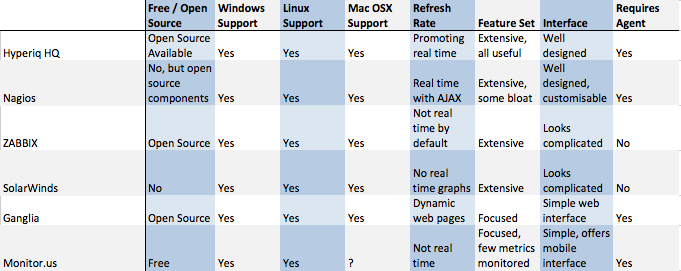
\includegraphics[width=110mm]{Competitors/MarketSurveyTable}
\caption{Overview of some of the systems we looked into}
\label{fig:SurveyTable}
\end{figure}

Figure \ref{fig:SurveyTable} shows some general findings for several frameworks that we looked into. We shall explore a selection of these further -- chosen to represent the diversity in functionality and usability in the table -- to get a better idea of where our own solution can fit among them.

\textbf{Nagios XI} \cite{nagios}

Nagios call themselves the industry standard in IT monitoring. This premium solution has a professional looking interface that gives power to the user, while remaining clean and useful.

Their dashboard, shown in Figure \ref{fig:NagiosDash}, keeps information clear for the most part, blue font on red background aside, and it is user customisable, so the user can choose what they see at the forefront of the application. This is a very useful feature, as Nagios boast many, many features and allowing the user to cherry pick the ones most useful to themselves makes the burden of wading through these feaures slightly less tedious after a while. But that is still a potential problem. For a user to discover useful functionality, they still have to find it first.

\begin{figure}[H]
\centering
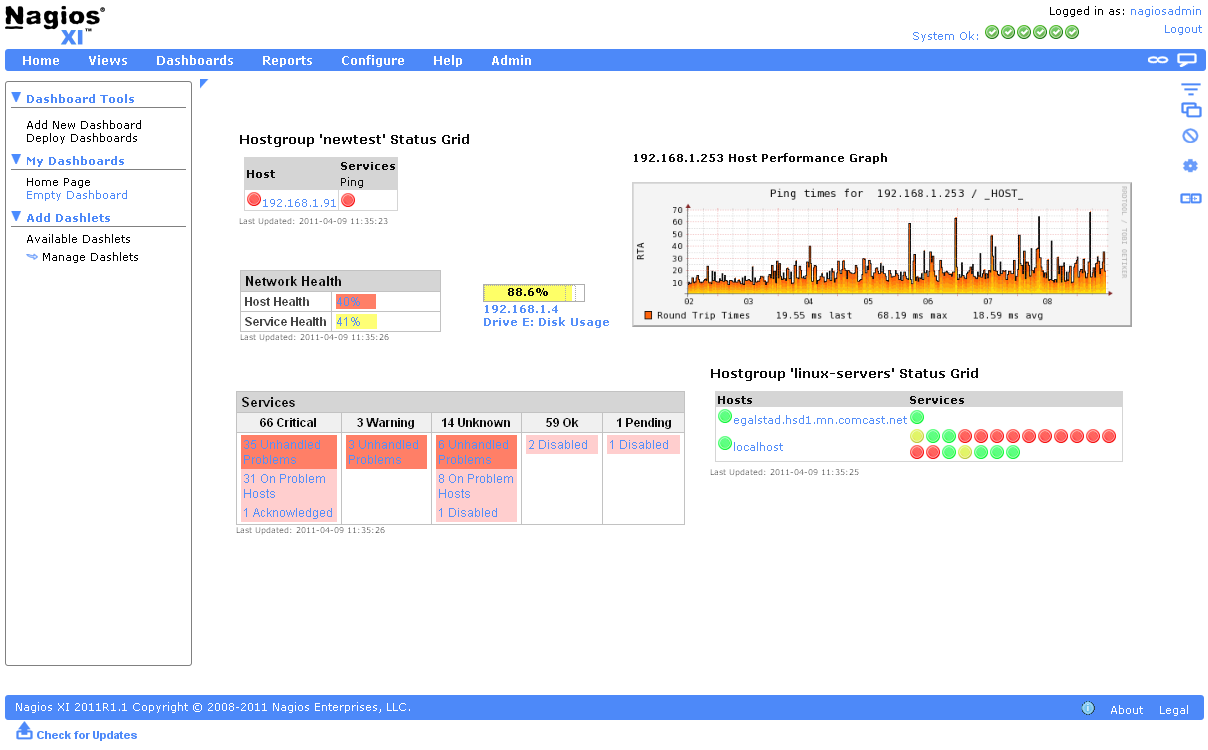
\includegraphics[width=110mm]{Competitors/NagiosXI_dashboard1.png}
\caption{Nagios XI's main dashboard view}
\label{fig:NagiosDash}
\end{figure}

What does this alert cloud in figure \ref{fig:NagiosAlertCloud} show? If, like the example pictured, you rely on IP addresses while monitoring, good luck untangling one set of numbers from the rest and then deciphering what its size and colour depict. Apart from being pretty like all alert clouds, this seems nothing more than a bullet point to pad out Nagios' extensive list of features.  It is unnecessary, and can confuse customers, an unfortunate side effect of having so many marketing points.

\begin{figure}[H]
\centering
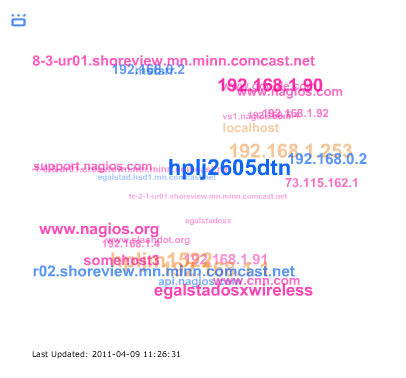
\includegraphics[width=110mm]{Competitors/NagiosXI_alertcloud.png}
\caption{Nagios XI's alert cloud view can't be much more than another bullet point}
\label{fig:NagiosAlertCloud}
\end{figure}

\textbf{SolarWinds Server \& Application Monitor} \cite{solarwinds}

Another monetised solution we explored was from SolarWinds. This takes the extensive feature set from Nagios XI and builds upon it with a cluttered and frustrating looking user interface.

\begin{figure}[H]
\centering
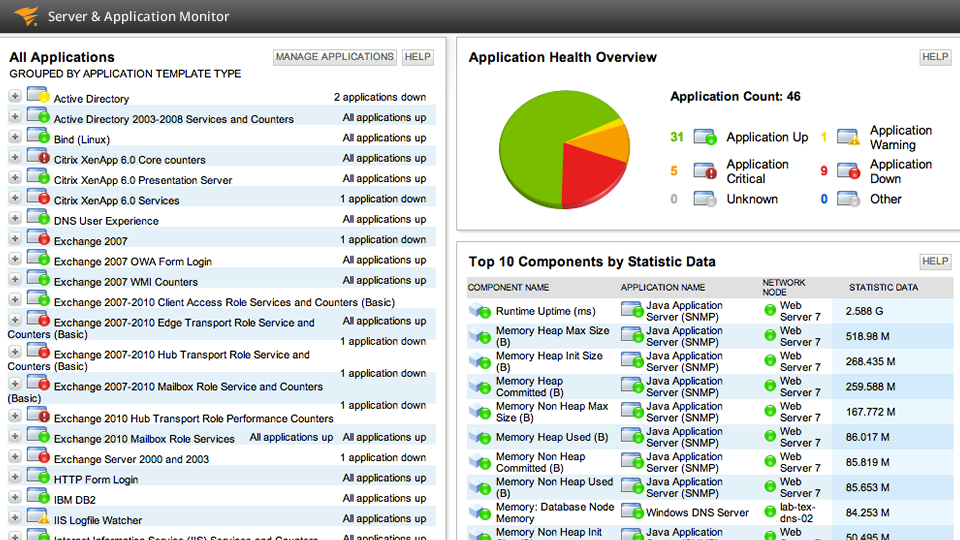
\includegraphics[width=110mm]{Competitors/SolarWinds_AppView.jpg}
\caption{SolarWinds' cluttered application view}
\label{fig:SWAppView}
\end{figure}

Screens are heavy on tables and have large numbers of rows each fighting for attention. Colour is used very sparingly, see in the top-right of Figure \ref{fig:SWAppView} that green and red, along with shape, are used in very small icons to signify applications that are okay or `down'. But being so small, shape can be hard to distinguish, and following one coloured icon's row in a block of similar icons could be confusing. The inspiration for our own interface so far has come from Nagios' solution.

\begin{figure}[H]
\centering
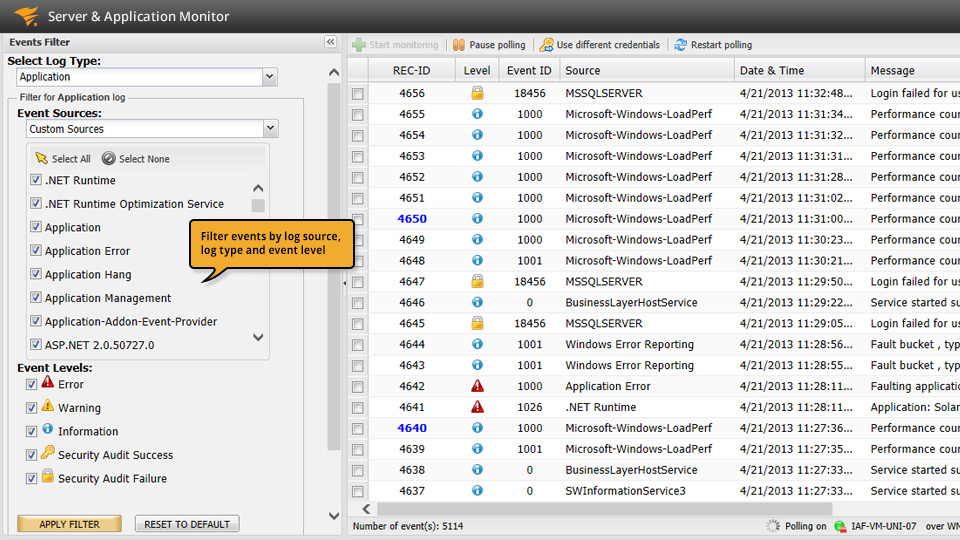
\includegraphics[width=110mm]{Competitors/SolarWinds_EventFiltering.jpg}
\caption{SolarWinds' filtering relies on the user scrolling through long lists of checkboxes}
\label{fig:SWFiltering}
\end{figure}

In Figure \ref{fig:SWFiltering}, see how SolarWinds promotes the ability to filter events, but asks the user to scroll through a long list of checkboxes in a rather small section of the screen in order to do this. Again, similar to Nagios XI, functionality has been thrown at the application and usability has been sacrificed as a result. Where Nagios XI has features that may not be useful, but seem to be implemented well, SolarWinds just overcomplicates what seems to be a powerful solution.

However, when reading reviews of the software, one user made an effort to emphasise that they really liked `Expert Knowledge'. Many performance counters gave a definition of the metric, an explanation of what the possible problem may be and suggestions of how to remedy the issue. This reviewer would be one of our own audiences; someone who may not know the ins and outs of their machines, but needs help when it comes to finding and rectifying problems. This kind of `helper' or `assistant' functionality could expand our potential user base to people such as this reviewer who aren't as knowledgable as the power users of some of these more expensive solutions.

\textbf{Monitor.us} \cite{monitorus}

Monitor.us differs from the previous competitors rather significantly. For one it is free and hence more of a direct competitor with our own solution, most likely being free as well. Second, it emphasises a mobile interface.\footnote{\raggedright{}Monitor.us' site did not supply screenshots for its desktop server monitoring solution. A side effect of this was the discovery of its mobile solution that became an interesting juxtaposition to the desktop solutions dicussed previously. However, as a consequence, some interface functionality is being implied from the screenshots.}

Phone interfaces must be simple. With less real estate to work with it is essential that everything displayed is clear and imperative that it be useful. While on a different platform, this mantra follows through to our own desired solution.

\begin{figure}[H]
\centering
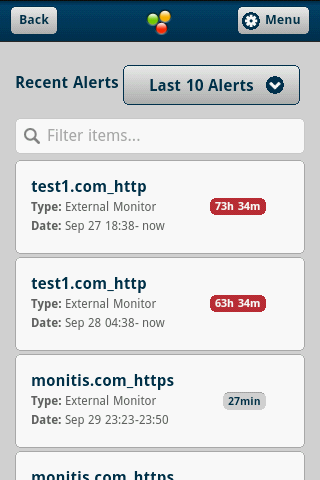
\includegraphics[width=55mm]
{Competitors/MonitorUS_iPhoneAlerts.png}
\caption{Monitor.us, a free monitoring solution, has a simple interface}
\label{fig:MUSiPhone1}
\end{figure}

In Figure \ref{fig:MUSiPhone1} you can see an interface for displaying recent alerts to the user. Before evaluating the interface, it should be noted that alerts were a feature not thought about by the team until conducting this survey. Indeed, many of our competitors promoted alerts -- notifications that a system metric has gone outwith a user defined ``safety band'' -- and it quickly became a feature we wanted to implement, making our own product even more useful.

The screenshot of Monitor.us displaying these alerts makes it instantly apparent that they have taken into account the smaller screen size. The number of alerts shown is limited to 10, so as not to bombard the user with information, and a drop-down selector can change this number. Also, to save scrolling, a search bar can be used to filter results without the kind of effort required in SolarWinds' filtering interface described in Figure \ref{fig:SWFiltering}.

\begin{figure}[H]
\centering
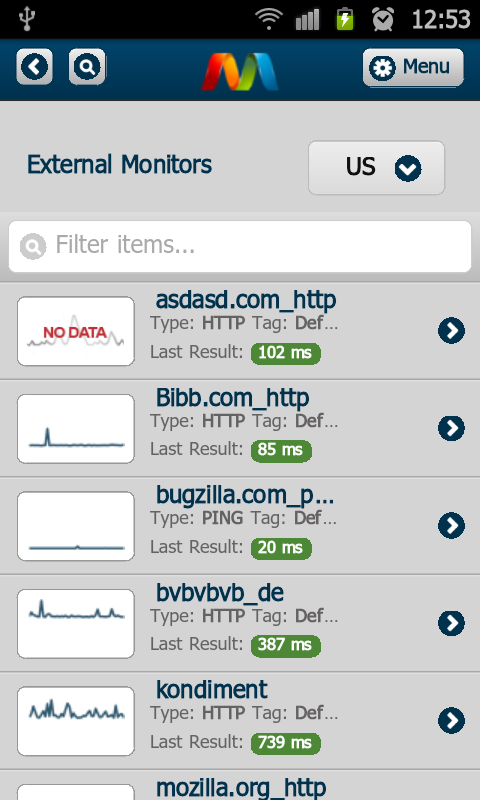
\includegraphics[width=55mm]{Competitors/MonitorUS_iPhone2.png}
\caption{Monitor.us uses its limited space well, in-line graphs allow for helpful info at a glance}
\label{fig:MUSiPhone2}
\end{figure}

The more standard view in Figure \ref{fig:MUSiPhone2} shows how a user might view the current status of any systems they wish to monitor. Screen size remains a design thought, with small -- but readable -- graphs showing past data that allow the user to get instant context concerning a system's recent history, and spot any anomalies they wish to look into further, most likely with a simple tap of the concerning icon.

However, being a free solution, Monitor.us does not promote real time data monitoring, but then neither did a lot of other competitors. It would seem that this is a feature that not many large companies have broached and again enforces that this be a key feature in our own product.

Ultimately, this prophet of simplicity, and our greatest competitor, would stress our aforementioned goals of simplicity and usabilty, keeping us focused on what is absolutely essential for our end users.

%-----------------------------------------------------------------------------------------------------------------------------------------------

\section{Market research findings}

\textbf{What should we monitor?}

Our competition offer literally hundreds of processes, events and hardware statuses to be monitored, some even offering hardware sensors that can be installed to monitor the climate in the client's server control room. While these are fun to think about, it quickly became apparent that this was a bullet point we simply could not compete with. Instead, we should focus primarily on gathering the most useful and relevant data that we can such as CPU data, memory stats, traffic etc as outlined in Section \ref{motivation}. We still have the potential problem of handling multiple operating systems, so biting off more than we chew is a real possibility otherwise.

\textbf{Competition has complicated interfaces}

Monitoring less stats also allows us the opportunity to really improve a feature that so many people seem to overcomplicate, UI. Offering so many things in one package makes our competition seem very bulky, non-intuitive and threatening. Lists upon lists upon graphs upon menus are displayed side by side and it seems a far from ideal layout. By working with the simplest data that the user needs, there is an opportunity for us to display graphs, allow for manipulation and offer customisation while still keeping this important information available at a glance, not hidden between tabs or scrolling panes.

\textbf{We should be able to set up alerts}

A common feature among similar products is the ability to set up custom alerts for specific data. Say the memory reached capacity and could have a potential knock-on effect to a company's customers, an alert could be set up so that memory was monitored and an email would be sent to the system admin (most likely via email) if it reaches a certain threshold. This also emphasises how critical it can be to have access to a server's system data with as little latency as possible and is an ideal addition to fulfill our brief.

\textbf{Predicting, preventing and repairing failures automatically is beyond us}

A more complex issue that links into the idea of alerts would be the ability for us to detect failures and problems without custom scripts or alerts. Many systems offer this functionality and some even promote their ability to repair failures automatically, however, this is beyond our own project.

\textbf{Potential for guidance if not automatic action}

SolarWinds had a review stating that many performance counters gave a definition of the metric, an explanation of what the possible problem may be and suggestions of how to remedy the issue. With our system aiming at smaller set ups, it's very likely that our user base will consist of novices, and such a feature could be highly useful. This of course presents the problem of showing information when it is needed to newer users, while also preventing it from becoming a nuisance to experts. This is a complex requirement, requiring an investment in time for both writing some sort of help documentation and then implementing it at a user interface level, allowing users to see this information on a metric-by-metric basis -- be that tooltips or an interactive first-steps guide.

\textbf{Closest competition has poor refresh rate}

Our seemingly closest competitor, Monitor.us, is a free solution that boasts a refresh rate of 30 minutes, its premium flavour reducing that to 1 or 5 minutes depending on how it is set up. Also boasting simplicity, it could be one to dig into more closely in order to discover how it handles its interface, a one dashboard view.

\textbf{We should promote simplicity at all stages}

Promoting simplicity and usability is definitely our main goal and so our solution should be just as easy to set up as it to work with. A short install time is something we will definitely be aiming for.

%-----------------------------------------------------------------------------------------------------------------------------------------------

\section{Summary}

With a clear idea of what our project should be, and having researched existing solutions that deal with similar problem descriptions to our own, we have identified more clearly what functionality our product must provide, as well as how it should present this functionality. The following chapter formally lays out these functional requirements and explores non-functional requirements that deal with the likes of scalability and performance expectations.

%===============================================================================================================================================

%===============================================================================================================================================

\chapter{Requirements}
\label{req}

From team discussions, as well as our market research, we constructed a list of requirements to be fulfilled during the progress of this project.

%-----------------------------------------------------------------------------------------------------------------------------------------------

\section{Functional Requirements}
\label{requirements}

%Requirements discovered that focus on a user's interaction with the saystem

%NOT OUR MOST RECENT REUIREMENTS, i.e. AFTER DISCUSSION WITH J.P.MORGAN

\begin{itemize}
  \item R1 -- Real time data flow with websockets
  \item R2 -- Start daemon
  \item R3 -- Stop daemon
  \item R4 -- Server stores data
  \item R5 -- Alerts
  \item R6 -- Historical queries
  \item R7 -- Change metric being monitored
  \item R8 -- Multiple graph types
  \item R9 -- Save historical queries to user's own machine
  \item R10 -- Customisable dashboard
\end{itemize}

\subsection{Requirements details}

\textbf{R1: Real time data flow with websockets} \newline
\textbf{Description:} Users should see graphs and daemon stats update in real time. \newline
\textbf{Rationale:} This feature is deemed a priority from our project brief and would set us apart from a lot of other free solutions already available, allowing users to react to problems as and when they happen. \newline
\textbf{Priority:} Must have

\textbf{R2, R3: Start and stop daemon monitoring} \newline
\textbf{Description:} Users should be able to start daemons after installation, and stop them when needed. \newline
\textbf{Rationale:} This is essential for a functional system. \newline
\textbf{Priority:} Must have

\textbf{R4: Server stores data} \newline
\textbf{Description:} The server should store some of the real time data points sent by the daemon. \newline
\textbf{Rationale:} This would allow for the user to query this data later. \newline
\textbf{Priority:} Must have

\textbf{R5: User defined alerts} \newline
\textbf{Description:} Users should be able to set up alerts that notify them of any anomalies in their systems when they are not using the app. \newline
\textbf{Rationale:} This can really take advantage of our real-time data so users are notified of anomalies when they happen, and not minutes or hours later, allowing them to try and rectify the problem. Identified from market research. \newline
\textbf{Priority:} Should have

\textbf{R6: Historical queries} \newline
\textbf{Description:} Users should be able to look at past data stored by the server. \newline
\textbf{Rationale:} Users could look for trends in previous data that allows them to predict future events. \newline
\textbf{Priority:} Should have \newline
\textbf{Dependencies:} R4

\textbf{R7: Change metric being monitored} \newline
\textbf{Description:} The user should be able to choose what metrics the daemon sends them, and what graphs they currently wish to see. \newline
\textbf{Rationale:} This gives some power to the user and makes sure they are seeing what they want to see, when they want to see it. \newline
\textbf{Priority:} Should have

\textbf{R8: Multiple graph types} \newline
\textbf{Description:} The user should be able to select how they see their data. \newline
\textbf{Rationale:} Some graphical views are better at gleaming certain information from data than others. Give the user the power to choose. \newline
\textbf{Priority:} Could have

\textbf{R9: Save historical queries to user's own machine} \newline
\textbf{Description:} The user should be able to store a view of their past data. \newline
\textbf{Rationale:} Being an open source solution, it would not be feasible to allow our server to store user data indefinitely, so the resolution will decrease over time. Users should have the option to store past data themselves should they wish it. \newline
\textbf{Priority:} Could have \newline
\textbf{Dependencies:} R4

\textbf{R10: Customisable dashboard} \newline
\textbf{Description:} The user should be able to choose what they see upon start up. \newline
\textbf{Rationale:} Different users want to monitor their machines for different reasons. Allow them to instantly get to the information they need. \newline
\textbf{Priority:} Would like to have

%-----------------------------------------------------------------------------------------------------------------------------------------------

\section{Non-functional requirements}
\label{nfrequirements}

%Requirements discovered that focus on how the system should perform while being used

\subsection{Server requirements}

The emphasis for the server is on the horizontal scalability. It has to provide concurrent access for multiple users from multiple organisations to multiple daemons. Even if the only company running the application will be J.P.Morgan, they have a few thousands developers in the UK, organised in lots of different teams, that would most likely be represented as organisations in our application. From our interview with them we have learned that the teams there have an average size of 9 people. We will round up that number to 10. We will assume that on average they would have to monitor up to 100 different clusters, though in reality a few teams will have massive ones, and the rest will probably require only about 10 instances. Overall, the requirements then would be:
\begin{enumerate}
\item it has to support 1000 concurrent users,
\item belonging to 100 different organisations,
\item monitoring 10000 different daemons.
\end{enumerate}

We feel that these requirements outline a reasonable scenario describing a moderate usage by either J.P. Morgan alone or a hundred middle-sized companies. We hope that we can provide this support while staying as low on resources as possible.

\subsection{Daemon requirements}

Due to the fact that the daemon is meant to run constantly in the background on monitored machines, the focus was on keeping it small and very fast while providing all the required monitoring and communication features.

Furthermore, due to the variety of platforms clients would like to monitor, the daemon must be easy to deploy and develop for most platforms.

Internally, the daemon needs to send data regarding all the monitored parameters to our central server, as well as all clients that are currently connected to it for real time data gathering. To do this, the daemon has to implement a common communication protocol, initiate a connection to the server, and accept any number of connections from clients.

%-----------------------------------------------------------------------------------------------------------------------------------------------

\section{Summary}

Defining these requirements provides clear goals for the project both in terms of functionality and performance. It also makes it easier to design how our solution should be built. 

%===============================================================================================================================================

%===============================================================================================================================================

\chapter{Design}
\label{design}

The following chapter discusses initial ideas and decisions that would go on to effect our implementation strategy. We will provide you with the architectural details as well as the motivation for certain choices.

%-----------------------------------------------------------------------------------------------------------------------------------------------

\section{Overall system}

\subsection{High level design}

\begin{figure}[H]
\centering
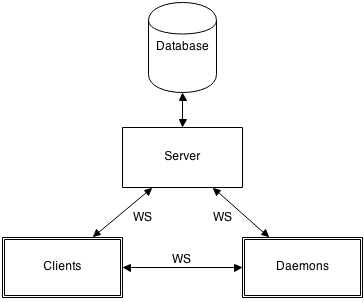
\includegraphics[width=110mm]{images/ArchitectureDiagram.png}
\caption{Overall Architecture Diagram: Main Components}
\end{figure}

We decided that the best way to tackle this problem was to split it into three main components and a database.

At the center we have a single web Server. It acts as a broker between the Client and the Daemon in order for them to establish a connection, as well as storing historical monitoring data that the Daemon sends. All the control messages that the Client might want to issue to the Daemon will also go through the Server.

The Client is a web application that shows real time performance data from the Daemons. In order to do so, it directly establishes a websocket connection to one or many Daemons, with the help of Server. It can also retrieve historical data for any given Daemon that it has access to from the Database through the Server.

A Daemon is a small application that runs on the machine and monitors its performance. It sends the data that it gathers to one or many Clients in real time using websockets, and it also stores sparser data points in the Database through the Server. It can be told to monitor different things, and these commands come through the Server.

Such separation of concerns flows naturally from the description of the task. It also enables us as a team to develop multiple independent parts in parallel.

A key to success in this case is the communication API. All three components implement the fully documented API, which ensures painless integration of the components, as long as the API is developed before them. The messages are being transferred using \texttt{WebSockets}, which reduces the excess data to transfer, reducing the network load and strongly improving the responsiveness of the application.

\subsection{API}

We have decided on a common \texttt{json} API, that had to be used for the communication between different components. All three of them had different commands, because of different functionality that they were implementing, but the commands themselves followed the same pattern of a command name and the data object, containing specifics. We attach the full description of the API in Appendix \ref{API}. 

We have chosen \texttt{json}, since it is much more concise than \texttt{XML} and is supported in \texttt{JavaScript} natively, as opposed to \texttt{YAML}, both of whom were alternatives. It also had really good libraries for \texttt{Go} and \texttt{C++}, reducing the cost of development. Moreover, it seems that \texttt{json} has become an industry standard for data interchange, pushing out \texttt{XML} hegemony\footnote{\raggedright{}JSON vs XML: \url{http://www.json.org/xml.html}}. 

\subsection{The technology}

The Client is a web-based application written in \texttt{HTML5}, \texttt{CSS3}, and \texttt{CoffeeScript}. The libraries used are \texttt{Backbone.js}, \texttt{Marionette.js}, \texttt{jQuery}, \texttt{Chart.js} and \texttt{Bootstrap}.

The Server runs on Linux and is written in \texttt{Go}. It uses a \texttt{MongoDB} database for storing the data.

Daemon can be compiled to target multiple platforms and is written in \texttt{C++}.

\subsection{Motivation for the choice of technologies}

\textbf{HTML5}\footnote{\raggedright{}HTML5 standard description: \url{http://www.w3.org/TR/html5/}} is the most modern standard for a markup language which is supported by a huge number of web browsers. This is the de facto standard technology, and hence a sensible choice.

\textbf{CSS3}\footnote{\raggedright{}CSS3 W3C introduction: \url{http://www.w3.org/TR/2001/WD-css3-roadmap-20010523/}} is a style sheet language that is used to describe the look of the document. Much like \texttt{HTML5}, it is a standard for the modern Web. At first we thought about using \texttt{LESS} (which in turn would be compiled to \texttt{CSS}) as it introduces some nice features like variables, nesting, loops and functions. However, due to the fact that there would most likely be more negatives than positives when introducing a language not many were familiar with, it was decided to stick with the standard.

\textbf{CoffeeScript}\footnote{\raggedright{}CoffeeScript's homepage: \url{http://coffeescript.org/}} is a language that compiles to \texttt{JavaScript}. The main motivation to use it was the opportunity to learn something new. It adds some syntactic sugar to\texttt{ JavaScript} which greatly improves the speed of development. Some of the team members started to use \texttt{CoffeeScript} in their daily development tasks.

\textbf{Backbone.js}\footnote{\raggedright{}Backbone.js documentation: \url{http://backbonejs.org/}} is a model-view-presentation framework for front-end development. Together with \textbf{Marionette}\footnote{\raggedright{}Marionette.js documentation: \url{http://marionettejs.com/}} it gives a very simple way to build large client-side applications. This framework was ideal for us, as it offers a huge number of features for single-paged apps. Similar to \texttt{CoffeeScript}, choosing this framework was motivated by an opportunity to learn a new programming paradigm and expand our toolkit.

\textbf{jQuery}\footnote{\raggedright{}jQuery: \url{http://jquery.com/}} is a library that massively increases the speed of web development. We cannot even imagine developing a large application without using this as it offers an enormous amount of useful shortcuts. Many team members know from experience that working with \texttt{DOM} directly always takes much more time than using \texttt{jQuery}. Also, it minimizes the differences in browser behaviours.

\textbf{Chart.js}\footnote{\raggedright{}Chart.js: \url{http://www.chartjs.org/}} is a library that is great in drawing data-driven charts. In our case it is responsible for presenting all the graphical information.

\textbf{Bootstrap}\footnote{\raggedright{}Bootstrap: \url{http://getbootstrap.com/}} gives us a fast way to make the application look similar on every platform. Also, it makes the user interface absolutely platfom-independent, both on mobile and desktop devices.

\textbf{Go}\footnote{\raggedright{}Frequently asked questions about Go: \url{http://golang.org/doc/faq}} was chosen for its potential to scale horizontaly\footnote{\raggedright{}A good summary of Go's advantages and disadvantages in one place: \url{http://stackoverflow.com/questions/2198529/what-are-the-advantages-and-disadvantages-of-go-programming-language}}. It has an extremely nice concurrency based on goroutines, which are sort of managed lightweight threads. It also features extremely fast compilation times, serving as a boost to development speed. Additionally, even though it is statically typed, it has a runtime that allows easy type assertion, and garbage collection, making writing \texttt{Go} almost as fast as using scripting languages (for those who know Go). Its closest opponent was Rust, which is a much more linguistically exciting language, but we decided to refrain from using it, seeing it as less mature.

\textbf{MongoDB}\footnote{\raggedright{Project's page explaining key MongoDB features: \url{https://www.mongodb.org/}}} is a NoSQL database, which was once again chosen due to its immense horizontal scaling abilities. It is relatively mature at this point with an ever increasing online community and good documentation, thus it seemed to be a fair choice, knowing that we will have vast amounts of loosely structured data to deal with.

%-----------------------------------------------------------------------------------------------------------------------------------------------

\section{Client application}

\subsection{Goal}

The web application has to provide an intuitive way of viewing how the remote machines are using their resources. The client does not have to know anything about the monitored machine --- they just need to see the information about it. The user interface should provide an opportunity to display this information in real time as well as the history of usage for a specified period of time.

On top of this data-centric display, the application should be capable of providing some implicit information. For example, if the daemon does not appear in the list of registered daemons, or it states that it is not active at the moment, the user should be able to recognise this in order to check if the machine is running correctly, or if it has an internet connection. One useful feature of the system would be the ability to send alerts to the user, an alert popping up whenever an abnormal activity is detected, most likely this could be implemented as an automated email. The application must also provide an easy process of new user and daemon registration, with users potentially neeind to perform this operation multiple times.


\subsection{Flow}

All the client-server and client-daemon communications are done through WebSocket messages. A single HTTP GET request is sent to receive the application and from there, once the user interface is loaded, a single, self-restoring WebSocket connection with the server is established. As the WebSocket API provides a method ``onclose'', we will know if and when the connection is lost. In this case a timer is created and after a short timeout a new connection attempt is made.

Once a client-server connection is established, the user implicitly sends a ``login check'' message that contains a session id cookie. The server can respond with two kinds of answers. The first one is an error message, that indicates that the server does not have any information about the cookie provided or that the session has already expired. In this case the application answers by changing the current view to the login page. Another answer indicates that the user is logged in. In this case the current view is changed to the home view of the application.

The login page has a standard form with login and password fields. When the required information is provided, a message to the server is sent. If the password matches the specified user name, the user receives a new cookie and some more information about himself and the view is changed to the home view. On error, the login page remains, with some message to the user saying that their login attempt failed.

After a succesful authorization (cookie or login), a ``daemons'' request is sent, the answer to this request being a list of daemons associated with a requesting user. Every element of the list contains some basic information about a daemon and to get more specific information the user should send another request called ``daemon'' including this daemon's ID. The reply to this request is simply a list of further information, including the address, specific to the desired daemon. When the address of a daemon is received, the connection is made instantly and the real time monitoring data is sent to the client. Now on every incoming message the corresponding data chart is refreshed to show the actual resource usage.

\begin{figure}[H]
\centering
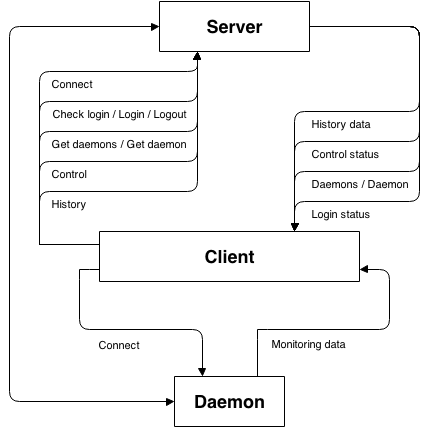
\includegraphics[width=110mm]{images/messages.png}
\caption{Message flow}
\end{figure}

\subsection{Components}

As we are using Backbone which is a mode-view-presenter (MVP) framework, the code is very nicely structured. Every component is a separate file written in CoffeeScript.

All the components can be split in groups:
\begin{itemize}
  \item UI components (views for tabs, daemons, charts, alerts)
  \item Model components (tabs, daemons, charts, alerts)
  \item Controlling component (controller.coffee - high-level callbacks and the daemon object)
  \item Service component (service.coffee)
  \item Framework specific components (Router, AppState)
  \item Communication component (Messages, Message Processor and Sockets)
\end{itemize}

\subsection{Concept designs}

Prototyping our user interface was an obvious task before doubling down on development. With the user experience such a prominent focus to the team, this would enable us to put ideas down on paper very quickly and inexpensively in order to achieve a clear and singular design vision in everyone's minds before proper development started. If executed properly, these designs should fulfill our user requirements of simplicity and usabilty, while also making development more focused and planned out.

When considering what would have to be evaluated with these designs, the primary goals were to:

\begin{itemize}
\item{Show appropriate information without crowding the page}
\item{Allow a user to navigate easily}
\item{Provide functionality described in our requirements}
\end{itemize}

When discussing these designs, the motives behind certain decisions will be explored alongside the proposed outcomes. This should build upon and solidify any of the requirements as specified in Section \ref{requirements}.

\begin{figure}[H]
\centering
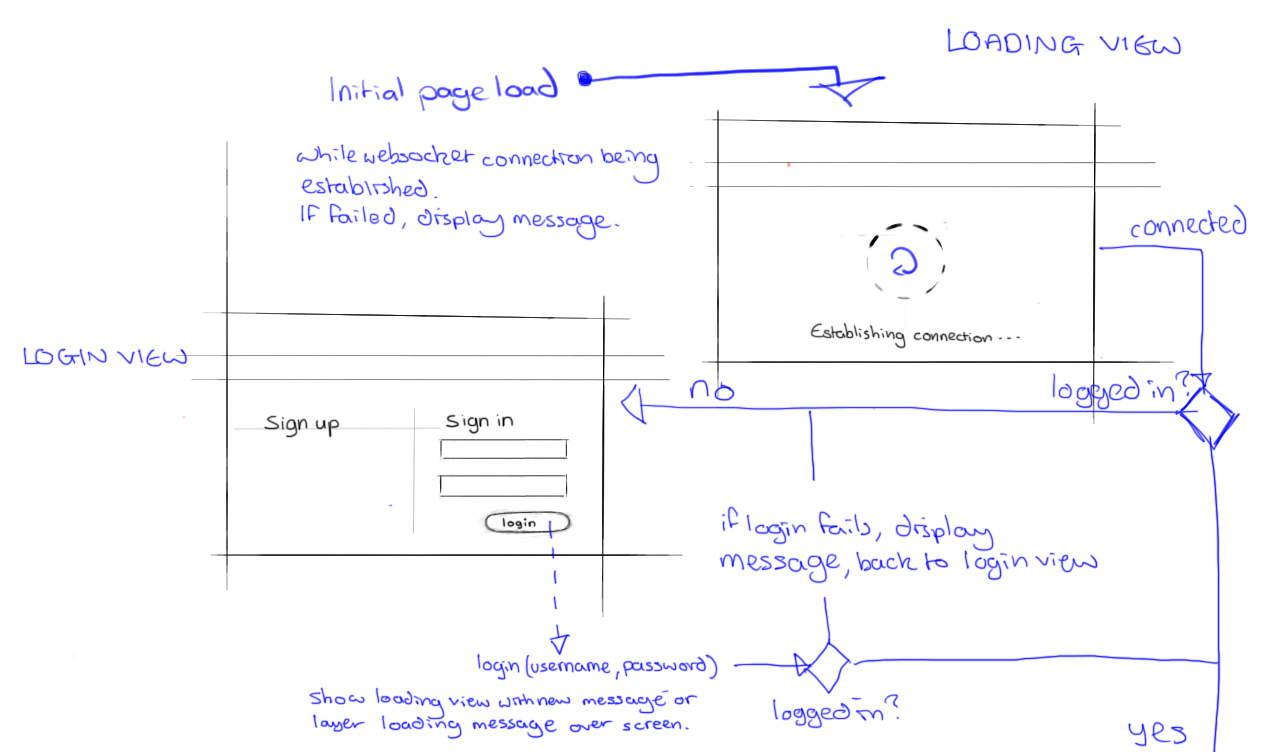
\includegraphics[width=110mm]{Concept_Designs/Login.png}
\caption{Login screen}
\label{fig:Login}
\end{figure}

The login screen shown in Figure \ref{fig:Login} should remain simplistic, and upon full completion may include some basic information about the project as a form of publicity or advertisement. However, the main feature explored here is simply the client's ability to establish a connection with our server.  With this project relying so heavily on information gleamed from the cloud, the user would have to be notified when the server was working to provide this information but there was nothing to see yet. So, on the login screen while a connection is being established, a spinner could be used with a simple message to keep the user informed of what's happening and why there may be any delay. This is a nod to the helpful and friendly user experience we aim to provide throughout the rest of the application.

In Figure \ref{fig:MainDash} you can see this spinner returning to inform the user that information is being accessed from the server, and there is currently nothing to see.  Obviously, any `loading' times should be reduced to an absolute minimum, but designing for the worst case scenarios and keeping them in-line with our best-case visions will hopefully unify the application and make it seem more professional, even when it stutters or fails.

\begin{figure}[H]
\centering
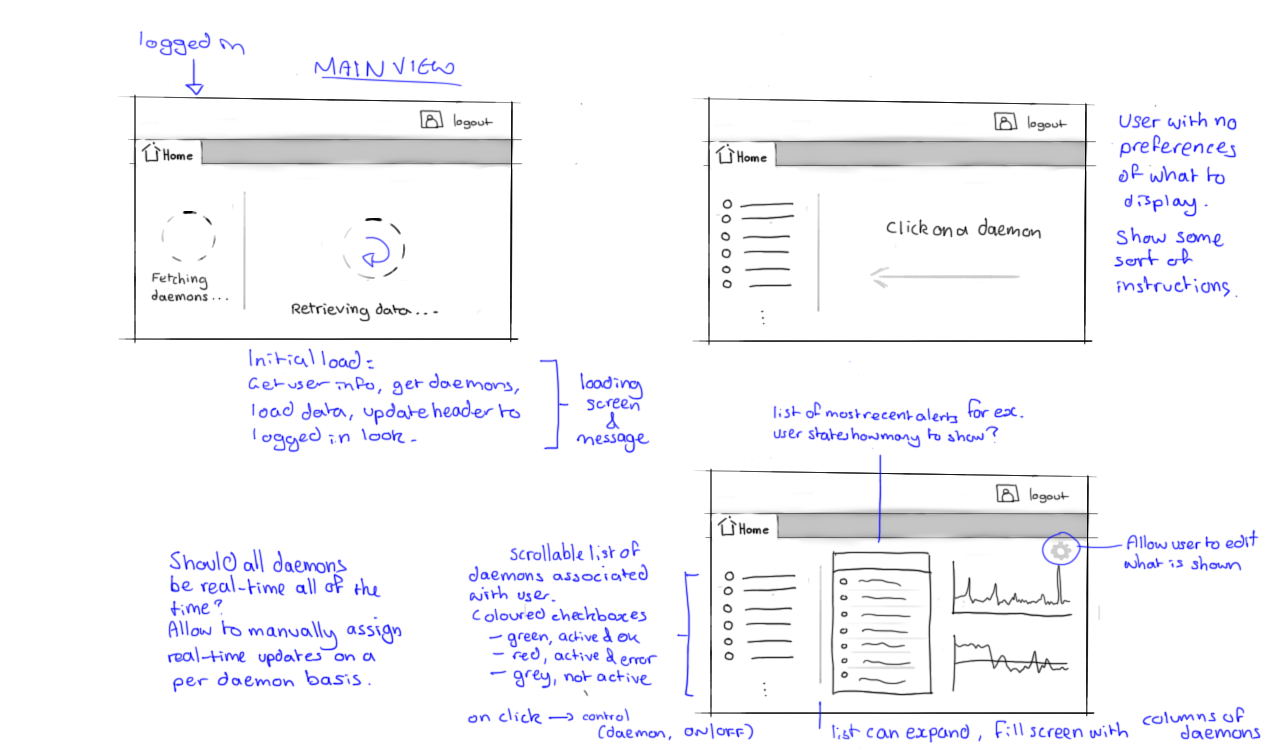
\includegraphics[width=110mm]{Concept_Designs/MainView.png}
\caption{Main Dashboard}
\label{fig:MainDash}
\end{figure}

To focus on some of the functionality now, there is a list of the user's daemons on the left side of the screen and a navbar at the top. These will remain constant once a user has logged in, allowing for a kind of visual anchor or safety net. As they navigate to different parts of the app, the header and sidebar should never really change much, so the user should not have to search around or relearn the interface when they switch between creating an alert or simply viewing the latest graphical data of a selected daemon. This was developed from our requirement of designing an app that is simple and clean.

The rest of the screen can be described as a content area.  Here, in the main dashboard, the initial idea was to allow for a user configurable space, where the user would choose what they wanted to see as soon as they logged in. In the bottom-right of Figure \ref{fig:MainDash} you can see an example layout where the user wishes to see a list of the most recent alerts for any selected daemon, along with two chart views of some metrics (perhaps CPU usage and network traffic). Again, this was developed as a counter to competitors' cluttered dashboards where one may get lost before they found what they wanted. This way a user could access their own most useful stats as soon as they logged in.

Now, let's say that a user has just installed daemons on their machine(s) for the first time, and are now logging in. The top-right of Figure \ref{fig:MainDash} shows this scenario being played out, with the content panel now providing instructions to the user on how to get started. Indeed, simply installing the daemons will not mean there is an instant connection to those machines and the client's interface in the final product. We have to provide some way of notifying the user that a daemon is not currently active. The solution is to colour code our daemon list, with grey icons representing inactive daemons that a user can click on to `turn on'. Similarly, green icons represent active daemons that are running without problem, and red icons represent daemons that are active but have encountered some kind of error, or the system they are running on is performing poorly. This information should help provide context to the user at a glance and allow them to make appropriate decisions quickly and easily.

\begin{figure}[H]
\centering
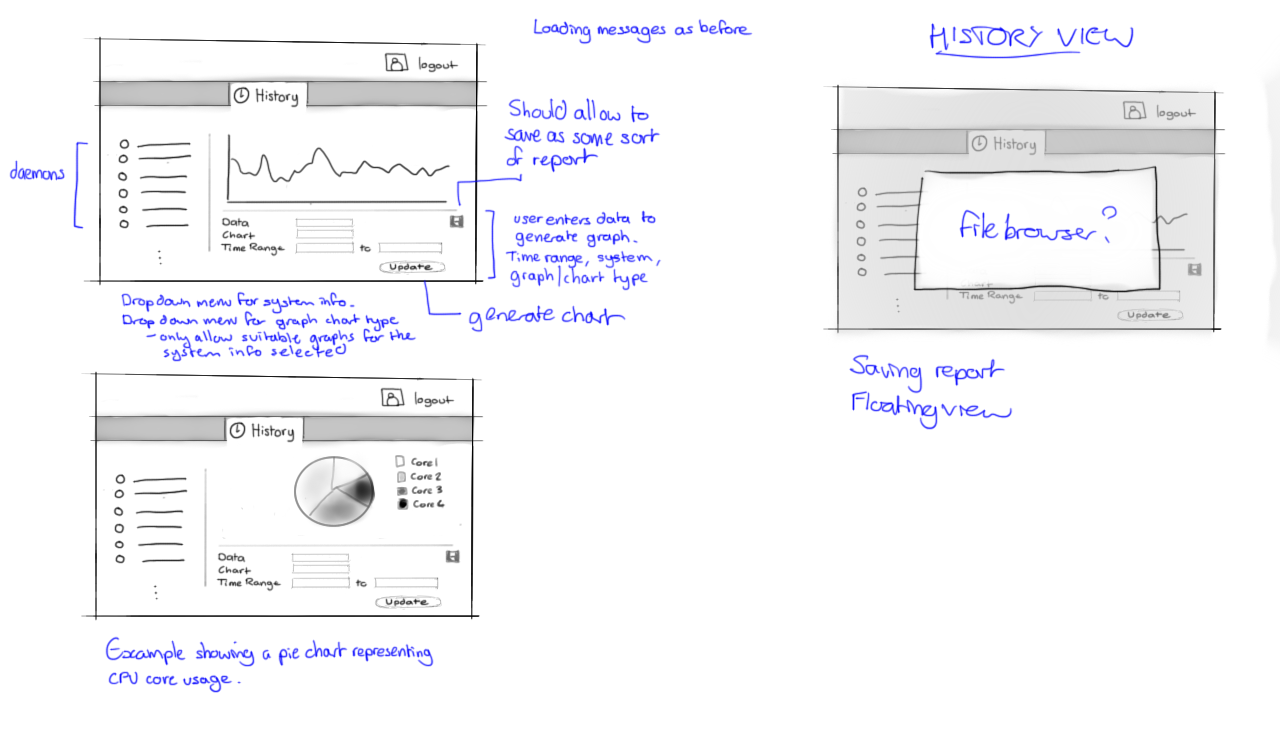
\includegraphics[width=110mm]{Concept_Designs/HistoryView.png}
\caption{History View}
\label{fig:HistoryView}
\end{figure}

When a user wishes to view past data stored in the server's database, they would click on the History tab. Notice how now, in Figure \ref{fig:HistoryView}, the header has changed to highlight the selected tab, so it is clear to the user where they are in the application. Also, the content panel has now changed to provide the functionality for this specific tab. Like before, a user selects the daemon they wish to query from the left sidebar, and then in the content view they can specify a specific metric's history to view as well as a time range.

Now with our project being part of our university coursework, this will likely be a free and open-source solution, and as such storing data indefinitely is completely unreasonable. Over time, the resolution of a user's past data is decreased in order to make room for high resolution recent data. But rather than just deleting old data and leaving it at that, it was decided that a user should be able to save a historical view of a daemon's data. In this history tab is a save icon to allow the user to do just that, perhaps bringing up a file browser for more control over what happens with the generated file.

\begin{figure}[H]
\centering
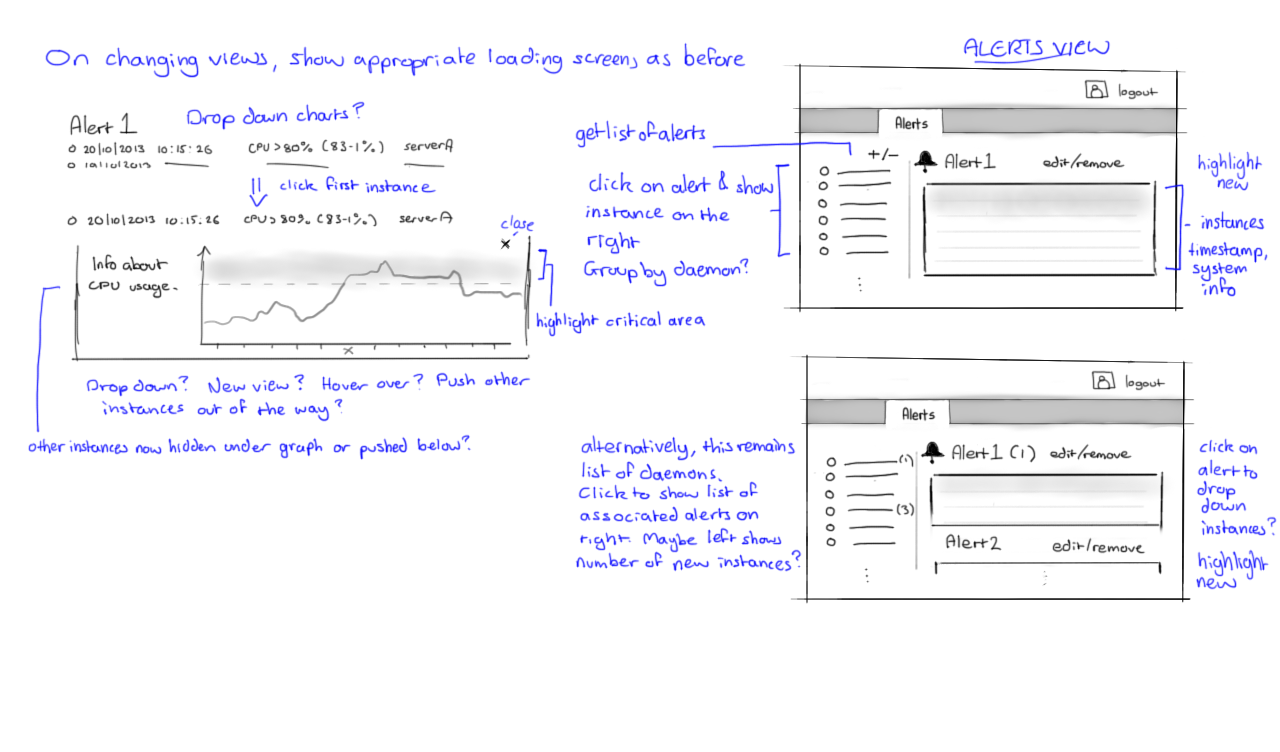
\includegraphics[width=110mm]{Concept_Designs/AlertView.png}
\caption{Alert View}
\label{fig:AlertView}
\end{figure}

As discussed in Section \ref{section:MarketResearch} concerning Market Research, the team thought it would be useful to provide user configurable alerts. Figure \ref{fig:AlertView} shows how such an interface might look like. This view houses a bit more complexity when it comes to development, as this is where a user would both see any instances of an alert having triggered as well as create new alerts.

Again, maintaining consistency, a daemon is selected from the sidebar and the content panel becomes a scrollable list of all the user-created alerts for this daemon. Underneath each alert, is each time the alert has been triggered, with new alerts that the user hasn't interacted with being highlighted so that they are instantly recognisable.

A more experimental design is shown in the top-left of Figure \ref{fig:AlertView}. Here, when a user clicks on an instance of an alert, a graph is instantly generated from, say, 30 minutes before the alert was triggered up to the current time. Essentially, this is a non-customisable, drop-down History view ala Figure \ref{fig:HistoryView}. It is providing instant context for the user about how their machine was performing leading up to the alert being triggered, and how it has continued to perform since. This could be a very useful feature to users but it does add difficulty to our implementation.

\begin{figure}[H]
\centering
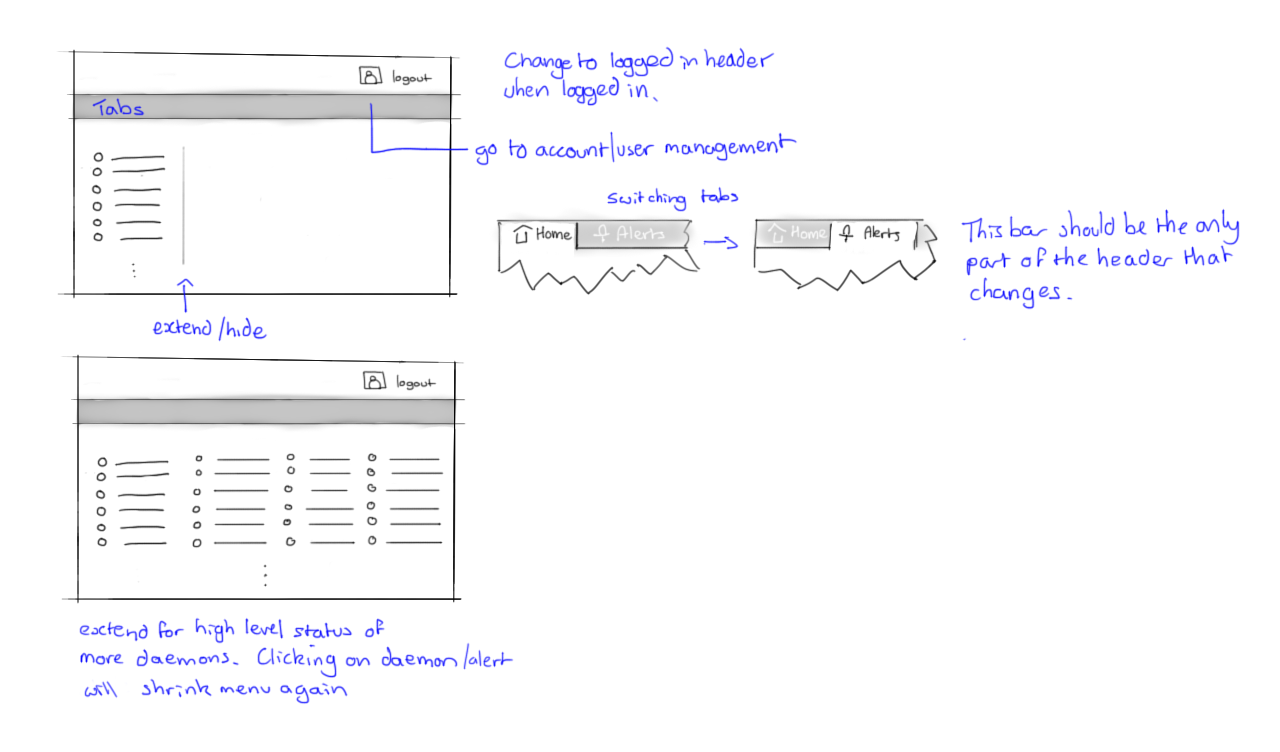
\includegraphics[width=110mm]{Concept_Designs/Misc.png}
\caption{Miscellaneous design features}
\label{fig:MiscDesign}
\end{figure}

Figure \ref{fig:MiscDesign} highlights some of the less feature-focused design considerations, such as the highlighted tabs being a way for the user to instantly know where they are in the application. Alongside this, it was considered that a user may have many, many daemons installed on multiple machines, so a small scrollable sidebar may not be useful all of the time. Hence, we designed a solution where the sidebar can be temporarily expanded to show a fullscreen list of daemons for the user to find the necessary one and select it, minimising the sidebar again. Here we also reiterate that this header is slightly different than when a user is logged out, showing user information, the option to logout, and the tabs.

%-----------------------------------------------------------------------------------------------------------------------------------------------

\section{Server}

\subsection{General overview}

\begin{figure}[H]
\centering
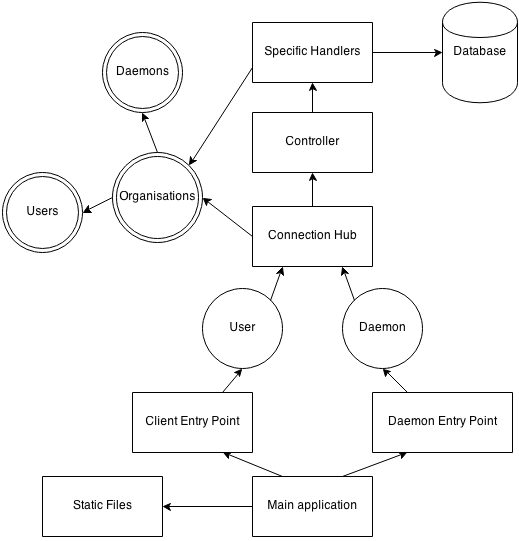
\includegraphics[width=110mm]{images/ServerDesign.png}
\caption{Design of the Server}
\label{fig:ServerDesign}
\end{figure}

While on first glance Figure \ref{fig:ServerDesign}, depicting the design of the server, might look very complicated, this is not really the case. The convention is that the rectangles represent key places in code, and the circles are entities (connections). Double circles just show that there are quite a few of them. 

Everything begins in the main application. This starts all the other parts, and this relationship is not shown to avoid cluttering the diagram. The main application registers handlers, starts an internal static content server (so that the client application can be reached), starts the connection hub and provides entry points for clients and daemons to connect to. Most of these things live in their own goroutines afterwards, and the main application just sits there, waiting for them to stop. In the following sections we will describe each of the components in the rough order of dataflow.

\subsection{Static content}

The main application sets up a file server that serves static content to the client. The client application itself is hosted here, being served together with all of its scripts and stylesheets.

\subsection{Entry points}

There are two entry points to this application, mapped to two different routes: `wsclient' and `wsdaemon'. Both of them are accessed via websockets and produce the same connection object that is to be handled by the connection hub. We need two separate handlers in order to attach an owner to those connections, because the application needs to differentiate between them. We show these connection objects as User and Daemon on the diagram, and they are being channeled to the hub via the register channel, in order to actually incorporate them into the application.

\subsection{Connections}

Connections are objects holding an open websocket, sending channel and an owner, which is either User or Daemon. There is a one-to-one relationship between owners and their connections. Once created, they result in two goroutines,\footnote{\raggedright{}a concept in Go, lightweight thread of sorts. The ``physical'' threads in the OS execute program instructions concurrently. A goroutine represents such a thread, but it is actually mapped to one by the Go runtime that manages a thread pool. Hence, Go is an example of managed concurrency.} one of which listens for the incomming messages and broadcasts them to the hub, and another sends messages back from the server to the client or daemon, depending on who created it.

\subsection{Connection hub}

The connection hub serves three purposes, accomplished via three different channels. It accepts new connections on the register channel and stores them internally. It authorises these connections and adds them to the anonymous organisation (more about organisations later). It also deals with closing those connections and removing them from the application, when it receives such a call on the unregister channel. Then it listens for the incoming messages from the currently open connections and forwards them to the controller. 

\subsection{Organisation}

The organisation is much like a namespace in the current design. It holds its own daemons and users, once they are authorised. It also provides a communication interface: all the daemons and users should only be accessed through the organisation object. It is a runtime tool – it only holds the currently active entries, however, it has its representation in the database, with which we can get all the users and daemons that belong to the given organisation. 

Authorisation, however, happens only after a certain request from the connection. Prior to that it lives in the anonymous organisation, a pre-created entity designed just for this use. While the connection belongs to that organisation, its reach is limited, as it can only execute handlers connected to proper authorisation.

\subsection{Controller}

The controller accepts \texttt{json} messages that are being sent by the connections, parses them, and executes their respective handlers, providing them with the message data. It knows which handler to use, because the main application has informed it of this by registering the handlers at the very beginning. When it fails to find one though, it returns an error message. Otherwise, it returns the result of the handler, which can be either an error object or null, so that the errors can be handled outside of the controller.

\subsection{Handlers}

Handlers implement a small piece of functionality associated with the particular API call. They are being registered by the main application, and invoked by the Controller, upon receiving the aforementioned call. They are being given an already parsed request as opposed to serialised \texttt{json}, and it is their responsibility to check whether the call adheres to the API, including the typechecks. Handlers return error objects for the errors they might encounter, which are then sent back to the requester from the hub as a special error message. In the case of a success, they themselves send the result messages, if any, to the connections involved.

\subsection{Database}

Using a NoSQL database (MongoDB) turned out to be a real challenge, since the principles of its design differ significantly from the relational databases that we were used to. While in the relational database one generally tries to achieve third normal form, in a NoSQL database one tries to denormalise data in order to match the usage pattern. Hence, we have identified two potential approaches to the problem: we could either design the database in a way that is easy to use for us and then provide the user with means of interaction, or we could devise the most sensible usage patterns and then adopt the schema to suit these needs. Being customer-centric, we have decided to stick with the latter option.

Hence, we have come up with the following database schema:

\begin{figure}[H]
\centering
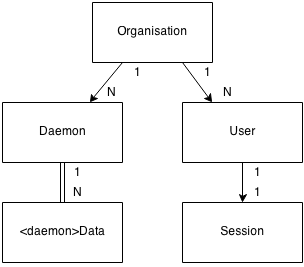
\includegraphics[width=80mm]{images/DatabaseSchema.png}
\caption{Database Schema}
\end{figure}

The diagram is self-explanatory end looks vaguely familiar: things in rectangles are collections, a rough equivalent of a SQL table, and I also show cardinalities of some relations. However, there is one NoSQL feat in this schema. Most of the relations are done in the regular fashion: Organisation has many Daemons and many Users, each User has one Session. Each daemon has many data points attached to it, and this is implemented in an unusual way – instead of having a foreign key that references the Daemon table, as we would do in a relational database, each daemon creates its own collection that has a name based on the daemon's name. MongoDB supports lots of collections in its namespace, so this allows us an efficient way to retrieve the data now that it is always available from the same daemon in one collection. In such a way we optimise for our usage pattern, since the user will usually want to see a piece of history from one given daemon.

%-----------------------------------------------------------------------------------------------------------------------------------------------

\section{Daemon}

\subsection{Overview}

The daemon's two most important parts are the watchers, which gather the information about the different parameters that are being monitored, and the connections, which communicate back and forth with the server and connected clients. A central manager handles them and ties them together.

\subsection{Watchers}

Each watcher is associated with one parameter that the daemon monitors. Currently, the watchers are:
\begin{itemize}
  \item CPU, which reports the overall utilization of the CPU as a percentage
  \item RAM, which reports the overall RAM utilization in bytes
  \item Network, which reports the total upstream and downstream added up, in bytes/second
\end{itemize}
These watchers are templates for platform-specific implementations, and are used by the central manager to get data in the same format without needing to worry about the platform the daemon is running on after the watchers have been created and started.
Generally, the structure of each watcher is similar: they begin running in parallel, getting the desired parameter every few seconds, according to the refresh rate they were set to, and they offer a way for the manager to retrieve the data resulting from that operation.

\subsection{Connections}
There are two asynchronous connection managers. The first one opens the connection to the main server, and allows any data to be sent to it from the main daemon manager, and the second accepts any number of connections from clients, and can simultaneously send data to all connected clients through the main manager.

\subsection{Main Manager}
This is the component that initializes and ties everything together. It synchronizes the refresh rates of the watchers, and sends messages to the server and clients through the connections.

%-----------------------------------------------------------------------------------------------------------------------------------------------

\section{Summary}

Our system is a moderately complicated one, and during its design, it has required us to make many non-trivial architectural choices. They may not be the best possible ones, but most of them are certainly sensible. We feel that a significant investment into the design at the beginning of the work saved us a lot of hassle in the long run. The relatively independent character of the components made it possible for us to streamline the development by tackling all of them in parallel, which proved to be largely successful. Read more about the implementation in the following chapter.

%===============================================================================================================================================

%===============================================================================================================================================

\chapter{Implementation}
\label{impl}

In this chapter, we describe the low level details of how the high level designs discussed in the previous chapters were used to construct our product. It will also feature some reflections on the overall development process.

%-----------------------------------------------------------------------------------------------------------------------------------------------

\section{Initial steps}

\subsection{Technology prototypes}
\label{prototypes}

% Our first attempts at creating a simple echo server, getting all the components to talk to each other...

Our first steps were directed at researching whether the technology choice was valid and would allow us to achieve the desired functionality. Based on our previous experience we decided that the trickiest part was to make all three components to communicate. We were unsure, whether the \texttt{WebSocket} protocol will be supported well enough in our target languages. Hence, we have decided to carry out a technology spike, if you like, and build a working prototype that does just that.

At the core of it laid an echo-server, multiple examples of which were found on the internet. The echo-server simply retranslates the message it receives, thus it is useful to see whether the connection comes through. To make it suitable for our tasks, we added the ability to distinguish between daemons and users, as well as to redirect the flow to each one of them. Most of that code was later reused for the Server part of the real application, and that is where the concepts of connections and the connection hub, explained in the design chapter, come from.

The client prototype had a very basic communication layer wrapped in a simple non-MVP based user interface. The first thing to do was to understand whether the \texttt{WebSocket} protocol is capable of sending a large amount of data for a long period of time and how browsers deal with that data. It turned out that the technology was quite capable. However, some browsers (primarily, WebKit-based) can have some memory issues when the data is sent for more than an hour (WebKit's garbage collector is known for its problems). In general, the client prototype proved that we are moving in the right direction. Later, a prototype proving the usability of \texttt{Backbone.js} was introduced. The final solution was built around the ideas and experience gained from making these prototypes.

The daemon, being based not on complex algorithms but on finding and understanding the ways in which the required parameters can be retrieved from different operating systems, started as a very simplistic version of the current design, with a tiny main manager starting a Linux CPU watcher - the first that was implemented - and outputting the data. The websockets library was quickly added afterwards, and a simple connection manager was created, which could accept one connection and could send the CPU data to that connection. We then used that to test the communication between the daemon and client, before starting to add more features.

%-----------------------------------------------------------------------------------------------------------------------------------------------

\section{Implementation of the client application}

\subsection{User interface}

User interface implementation is fully based on the approaches provided by \texttt{Backbone.js} framework and \texttt{Marionette.js} plugin. Every logical part of the UI is implemented as an independent Backbone model and a corresponding view. For example, a daemon is an extended Backbone model that implements a high level of daemon abstraction. It has some methods for controlling the daemon (starting, stopping, changing the metrics to monitor, etc). All the daemons are stored in a standard Backbone Collection. There is a View definition that is implemented as a Marionette ItemView that controls the way a single daemon is rendered on the page. The rendering is done by creating a template which describes what information has to be shown to the user. Also, the ItemView contains some event listeners that implement the processing of user actions (such as selection). Finally, there is a CompositeView (which is a part of Marionette) that describes how the whole collection of daemons is rendered. It has a template as well.

The same approach is used with tabs and charts.

\begin{figure}[H]
\centering
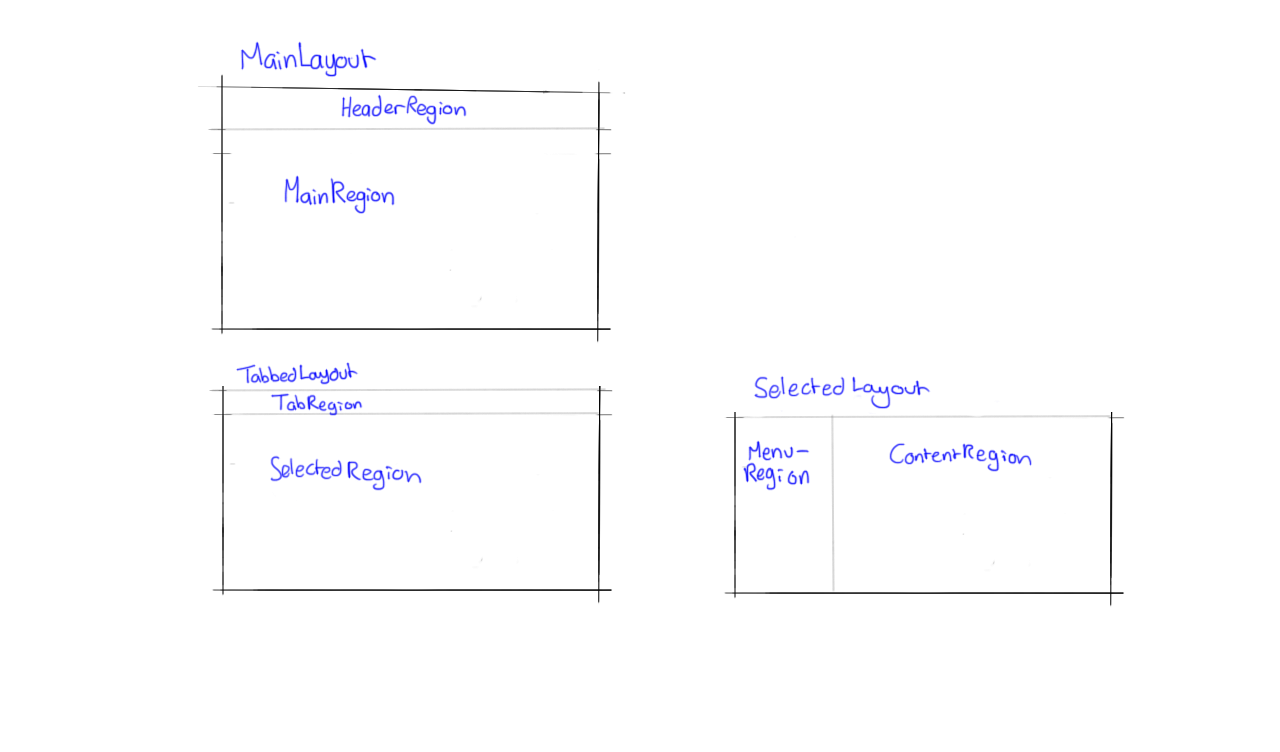
\includegraphics[width=110mm]{Concept_Designs/BackboneLayouts.png}
\caption{Backbone Layouts}
\label{fig:BackboneLayouts}
\end{figure}

In order to try and simplify the process of translating the concept designs to code, some templates were discussed that could be directly mapped onto Backbone's own templates. Figure \ref{fig:BackboneLayouts} shows these layouts, and also highlights how our design aims for consistency as much as possible, with switching tabs changing at most two regions, the ContentRegion and MenuRegion. This fact can be seen in the two example screenshots shown in Figures \ref{fig:Real-time data} and \ref{fig:History data}.

\begin{figure}[H]
\centering
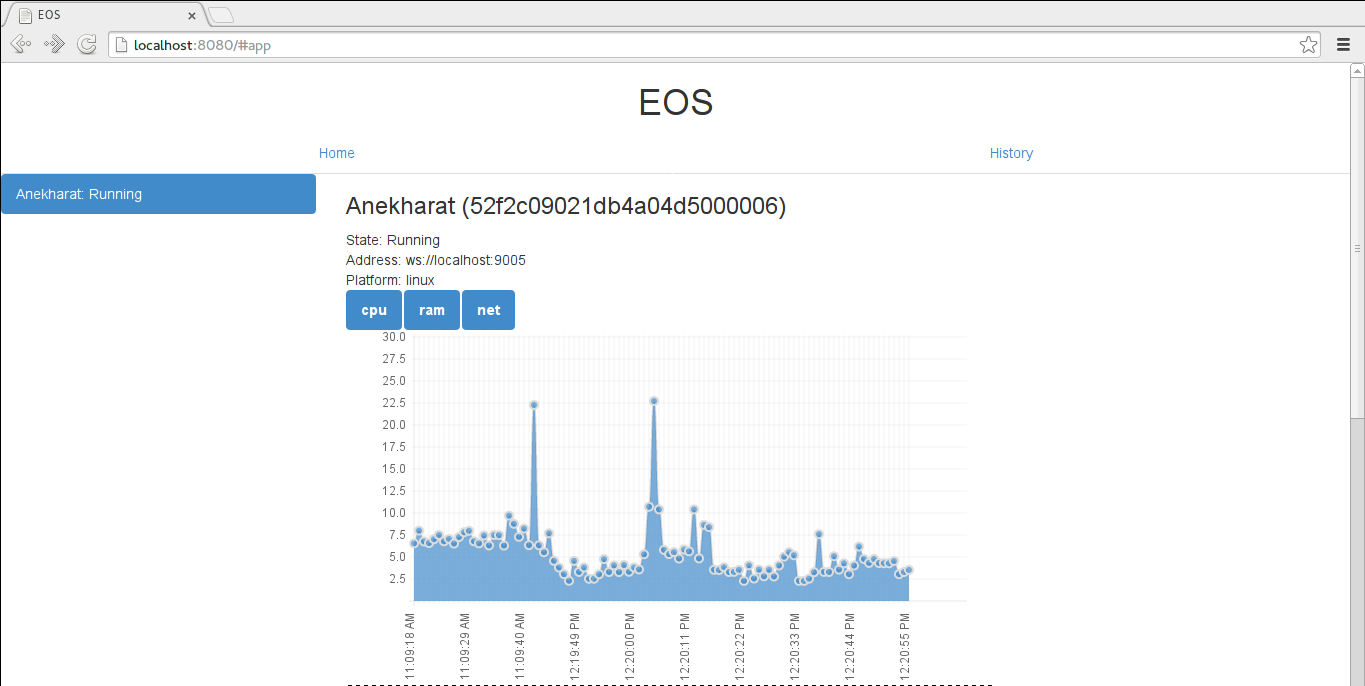
\includegraphics[width=110mm]{images/1.png}
\caption{Screenshot of the home view showing real time data}
\label{fig:Real-time data}
\end{figure}

\begin{figure}[H]
\centering
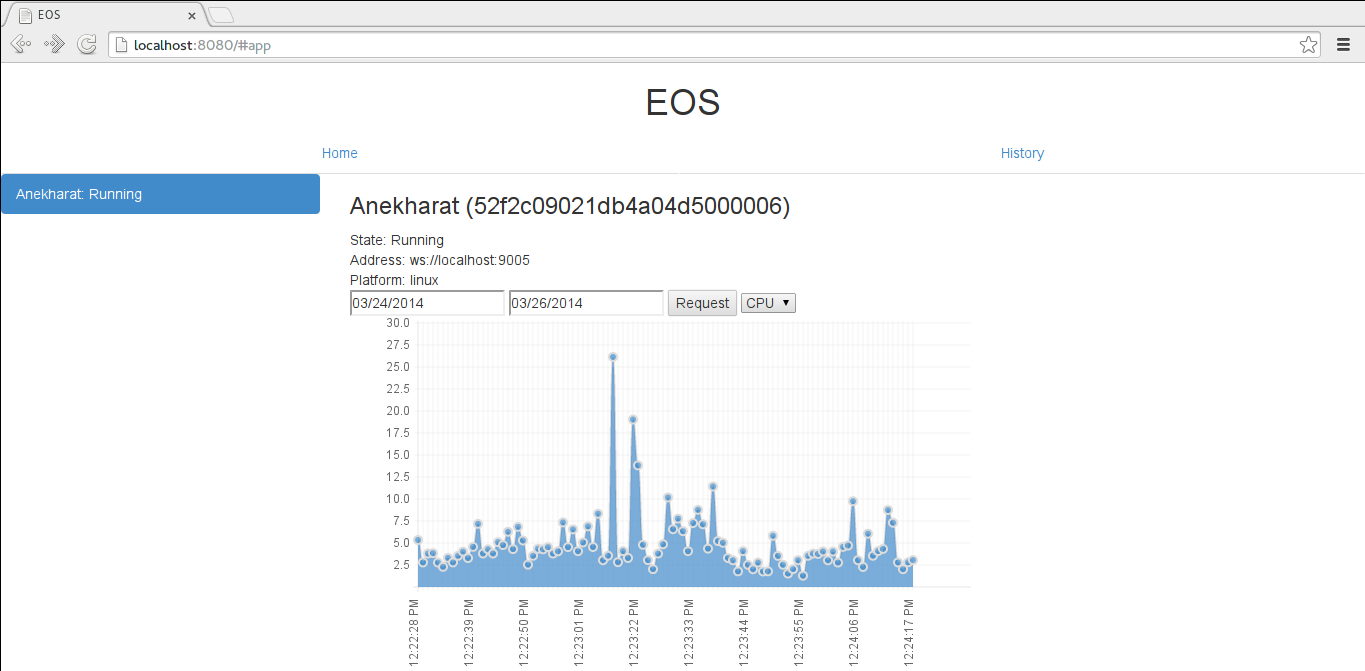
\includegraphics[width=110mm]{images/5.png}
\caption{Screenshot of the history view showing past data}
\label{fig:History data}
\end{figure}

\subsection{Communication}

One of the most important parts of the application is the communication component. It consists of the definitions of all the types of messages thst can be sent (which includes the data format and the callbacks for all types of requests), the message parser and validator. \texttt{Messages.coffee} describes a static class \texttt{Messages} which provides an interface for message creation, responding to the messages and their validation. Every incoming/outgoing message is checked by the helper methods to be well-formatted before processing/sending. This is done by the static \texttt{MessageProcessor} class. On an event of receiving a well-formatted message it is processed by an appropriate callback function (identified by the \texttt{Messages} class) which does the low-level data manipulations (such as identifying the error statuses and partial parsing) and then passes control to higher level listeners and processors. For example, if the user wants to send a ``control'' message to the server (the message specifies the id of controlled daemon and the action) the following things happen:
\begin{itemize}
  \item The message is created by a message processor which accepts the message type and its data, packs it into a JSON object, validates and returns it.
  \item The message is passed to the server's websocket send function that sends it using the native approach.
  \item The client has to wait for the response. It may not be instant.
  \item When the response is received, the incoming message is parsed and checked to be valid.
  \item The control is given to the callback that evaluates the answer and undertakes the corresponding actions.
\end{itemize}

\subsection{Sockets}

There are two types of sockets in the client application. The first one is the \texttt{ServerSocket}. It implements the interface provided by the standard WebSocket object. It is used as is without any wrappers. The second type is the \texttt{DaemonSocket}. It is implemented in the same manner as the first one except it has a bi-directional link with a corresponding daemon (which means that it ``lives'' inside the \texttt{Daemon} object and is meaningless without it). This socket can also be used to send data but this functionality is not used as our design assumes that all the client-daemon messages have to be deligated to the server. This improves the consistency of the states.

\subsection{Charts}

\begin{figure}[H]
\centering
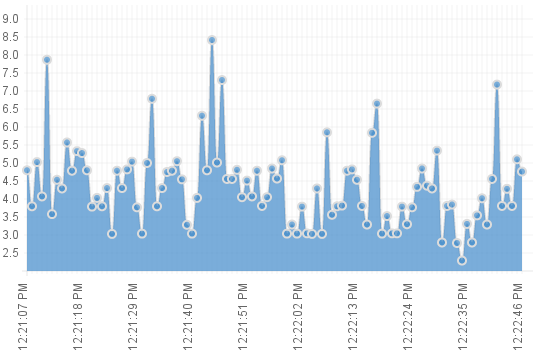
\includegraphics[width=110mm]{images/cpu.png}
\caption{CPU usage chart}
\label{fig:CPUusage}
\end{figure}

Charts are drawn on the HTML5 canvases that are passed as parameters for the \texttt{Chart.js} chart constructor. Each chart is capable of showing a history of a custom length (default is 100). For the history this value varies heavily as it depends on the data period selected.

Generally, there is a class called \texttt{Graph} which implements an abstract chart. There are classes for cpu, hdd, net and ram charts that extend the functionality of the base class. This implementation is separated as different metrics have different attributes. For example, the CPU count field can be introduced to the CPU chart to show the usage of each core separately. Similarly, RAM chart can have a maximum amount of memory. Each daemon stores a list of associated history and monitoring charts. On every incoming ``monitoring'' message the graphs are updated accordingly.

\subsection{States}

The components of the application and their different views should use shared data (for example, the current daemon). This could be done by introducing a number of global variables but Backbone offers a better approach. In our case an instance of \texttt{AppState} model is responsible for storing all the shared data. It does not only store the information, it is also responsible for listening to any changes to the data and firing all the necessary updates. For example, when the user logs in, the ``is user logged in'' flag is set to true in the controller. This event is immediately caught by an according listener and the current view changes. Here another component comes to the action and it is called \texttt{Router}.

\subsection{Routing}

\texttt{Router} is a standard method for handling the routes. In the use case described above, the Router's method ``navigate" is called. The AppState's listener passes the name of the page that has to be shown and two things happen. Firstly, routes changes the hash of the window's location object. This change is added to the history stack so the user is able to use the history object (which implies an opportunity of browsing the application using back and forward buttons). This also guarantees that the page can be bookmarked. Secondly, the Router executes a callback that is associated with the name of the requested page. In our case, when a user requests for the ``app'' page, the AppState's variable called ``current state layout'' is set to the new value. Here AppState's listeners again start doing their job - as the value has changed, an according action is performed - the page layout is set to the app's home view. Routing, together with objects like AppState, are extremely efficient in dealing with routing and shared data.

\subsection{Service}

There is a service component that provide some helper methods for working with cookies and some other things.


\subsection{Problems during development}

There were a number of non-trivial problems right at the start of the development. Firstly, none of the team members had any experience in working with WebSockets. This problem was solved in the most obvious way - we started to work with WebSockets. Gaining some experience did the trick.

Second problem was to overcome all the difficulties of Backbone (the framework has a steep learning curve). Again, intensive manual reading helped. However, there are still some unresolved bugs that are hidden under ``dirty hacks''. 

Another unpleasant surprise was brought by the chart libraries. It turned out that there is no library that can easily show more than 1000 data points at the same time. There is nothing we can do about it. On the other hand, it is a good reminder that showing too much information can be useless. If the system has to provide a lot of data points, they have to be presented in a nice way (showing 1000 points at a time is not a good idea).

Setting up a testing environment for JavaScript when writing in CoffeeScript using some additional libraries that imply following some specific programming paradigms is a huge problem. That's why we decided to do simple unit tests for the communication layer only. In general, it is enough because user interface can easily be tested manually.

Another difficulty was to test the existing code when other components were not ready yet. The solution to this was simple - the client prototype was able to send stub messages to an echo server. When the server responded, it's messages could be treated as the real message from the server of daemon.


\subsection{Stability}

Client-server and client-daemon connections restore if lost in the same manner. The development process has shown that the solution is able to provide real-time data for a very long time without any failures. Also, tests have proved that the client is able to work with multiple daemons at the same time and the incoming messages do not disturb each other. The only stability problem, as mentioned in Section \ref{prototypes}, can be the WebKit's memory usage.

\subsection{Testing}

The most important part that has to be tested is the communication. This includes testing the message creating / validation mechanism, sending, receiving and checking if the right callbacks are executed on incoming messages. These tests are done by creating a number of custom messages for each type of message and sending them to the actual development server. The answers are checked to be valid. The tests are implemented as a collection of messages, their expected responses and the methods that send these messages. No frameworks were used for this part and we wanted to keep the testing process as easy and fast as possible. The quality of the data that is used by the client is fully dependent on both the server and the daemon, because it does not generate any data itself (except control messages that change the state of a daemon), but only receives it.


%-----------------------------------------------------------------------------------------------------------------------------------------------

\section{Implementation of the Server side}

\subsection{The base}

The server inherited the core functionality from its echo-server prototype, such as the ability to receive the connections and serve static files. The code was cleaned up slightly, to enhance the integration of two connection types (user and daemon) as opposed to single. Other than that it was ready to be developed upon.

\subsection{Developing tools for testing}

We were developing three different parts to the whole system in parallel, and the development speed would vary, so we needed some tools to ensure that the server actually works. We have decided to take the test driven development approach because Go was an unfamilliar language and every little indication that what we were writing made sense would have helped us greatly.

Go comes with a testing framework, not unlike JUnit, out of box. It is implemented in the spirit of table testing, but table testing was of little help in this application. The application mostly communicates via messages and changes its internal state, so an enhanced ability to stub things would have helped. Unfortunately, Go lacked this ability, thus we had to create workarounds, mostly consisting of altering the real application state to create a specific environment, and then restoring it back to pre-test conditions. We have devised ways to insert temporary objects into the database, create stub handlers, and intercept sent messages during the testing. All of this allowed us to introduce acceptable levels of testing.

One controversial addition to the test harness was the Assert() method, that would abstract away the clumsiness of Go's test framework and provide rspec/jasmine style coloured output (see Figure \ref{fig:FailedTest}). While it made the work with the test harness much more robust and pleasurable, abstracting away Log() and Error() calls meant that the test harness could no longer tell on which line the error occured. It was still fine, knowing that every single Assert() message was unique-ish; nonetheless, if we had substantially more test cases this drawback might have slowed us down.

\begin{figure}[H]
\centering
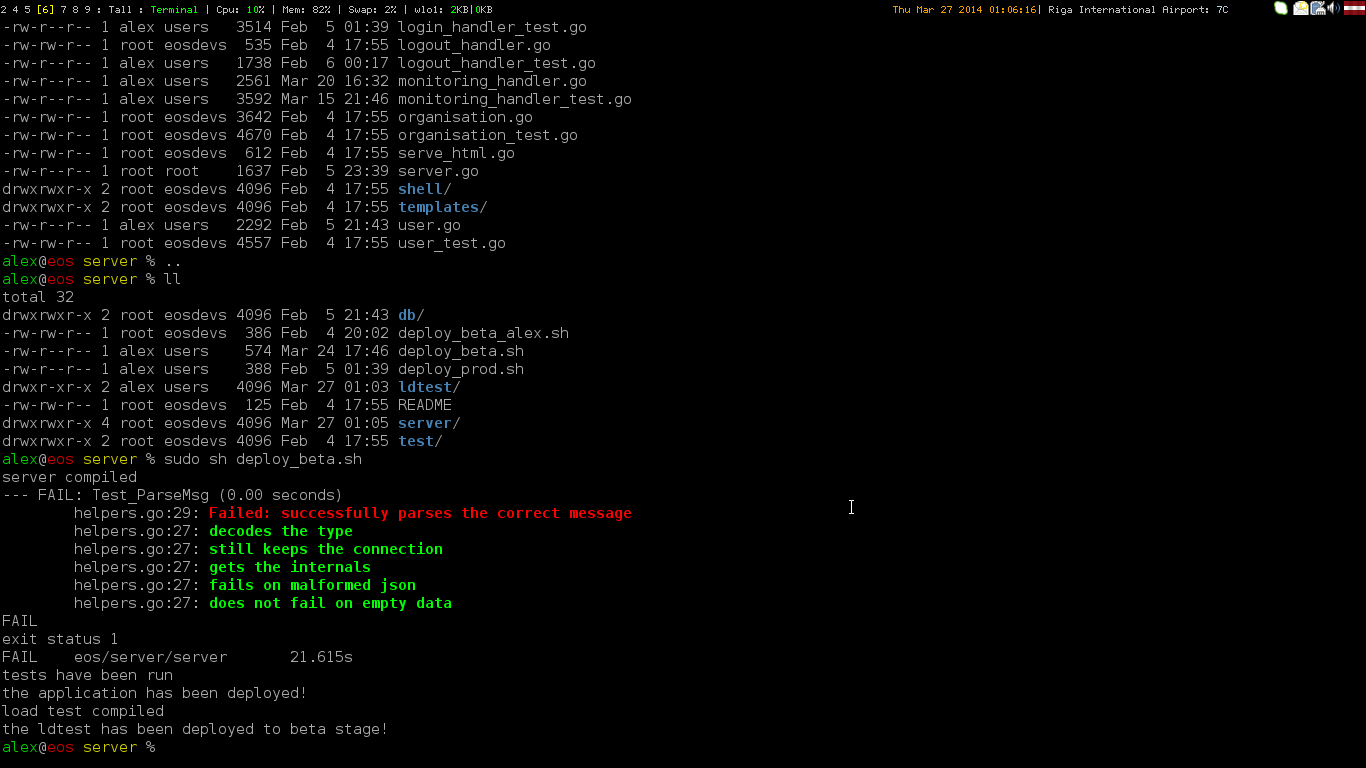
\includegraphics[width=110mm]{images/test.png}
\caption{A somewhat-artificial example of the failed test output}
\label{fig:FailedTest}
\end{figure}

Yet another issue was that we could not separate away test files from the main code, because that would have created some problems with namespaces. We could not resolve it at the time and we have felt that this made the sourcecode less clean, but this is more of an annoyance than a real problem.

Overall, introducing tests was a great success. Go' extremely fast compilation speed and performance testing framework allowed us to run tests before each deployment, and we have written scripts to do so. As a result of TDD we feel that we have a fair test coverage. While we did not run any test coverage tools (since they are officially supported starting from the Go 1.2, and for the Go 1.1 that we have used there is only a few broken ones to choose from), we cannot present a formal report on that, however, here are some fun statistics instead: 48\% of lines of code in the server package are in the test files and 11 out of 17 code files have tests. The remaining 6 files mostly feature old echo-server code, that was produced using StackOverflow-driven development, hence no tests. 

The tests vary in how much they follow unit test ideology: for controllers they are very much unit tests, but for handlers they are sometimes a sort of integration/regression/acceptance hybrids that are occasionally complicated, but other times just a variety of a smoke test. That is because we have clearly needed all of them, but did not have enough time to split them effectively. The usual development pattern was that we would TDD the code with unit tests, but after fixing some bugs that have slipped away, instead of developing real regression tests, we would transform unit tests into such, which we realise is flawed in the long term and ideologically punishable, however, it did give us immediate results with the least amount of effort. Also, I am yet to stumble upon an ideologically-correct project that features all these types of tests in perfect isolation while being developed in a chaotic agile fashion.

Despite all these problems, tests have done their job and the integration process with the rest of the codebase was indeed relatively painless. Hence, they were  a worthy investment.

\subsection{Creating the controller}

We have decided that the handler pattern would be most suitable for our needs here. The different API calls seemed to be quite independent from each other semantically (while sometimes required to be called in a particular order), and their list was by no means final. Having means to register handlers allowed us to be extremely flexible on the development of them.

The Controller part was relatively simple to write, since it turned out to be extremely testable. Being able to write comprehensive tests, we could develop it relatively quickly, rapidly fixing any arising problems. 

\subsection{Implementing each separate handler}

Each handler was developed separately. The most problems have arisen due to Go being a strongly typed language, while JavaScript, that was producing json requests, is not, and hence it was sometimes difficult to parse the message into correct types. In fact, this error was so common, that we had to abandon idealogical unit tests and expand them to cover parsing from actual json (which was tested in the Controller and was definitely working), because the parsed result was sometimes not what we would have expected, leading to the aforementioned ideological mess.

\subsection{The database}

The \texttt{mgo} library, that allows us to use \texttt{MongoDB} in \texttt{Go} is a beautiful piece of code, and in words of a 10gen employee: it might as well be the most advanced \texttt{MongoDB} driver out there\footnote{\raggedright{}As boasted by the mgo website: \url{http://labix.org/mgo}}. Thus, the integration with the database was painless: we had to create data structures that would represent different types of documents inside of the collections and then we could use them easily with \texttt{mgo} calls. In our opinion, the key to success of \texttt{mgo} was its documentation. It was of the highest quality, and almost completely eliminated any necessity to search anywhere outside of it.

An interesting observation was that \texttt{Go} being statically-typed, and thus its structures following the described pattern, while \texttt{MongoDB} is schemaless, was not a big disadvantage. In fact, since \texttt{Go} would just ommit the unrecognised fields in the documents, we could easily inject testing information there, creating ``stub'' objects in the database that could be easily deleted via a single query, while to \texttt{Go} they would seem real, allowing us to carry out extensive testing.

If by this time it feels that there is a disproportionate focus on testing in the chapter about implementation, it is intended, as it reflects the reality: making the code testable was the hardest part of writing the server.

\subsection{WebSockets}

Once again, the \texttt{Go websocket} library made  using this technology seamless for the most part. It was expected, since at the current stage the application has only the most basic utilisation of websockets: it does not go beyond standard send/receive scenario with default parameters. This was acceptable for the immediate goals of the application, since the security was not a priority.

During the development of the echo-server prototype, the Server connected to the Client easily. However, there were problems with the Server-Daemon connection: we were not able to establish it. Our first thoughts were that the aforementioned library did not send the required headers, since after inspecting its source code we have found quite a few TODOs in the code that were responsible for this. It turned out that we were wrong, and the problem was actually in the \texttt{Websockets++} library. In any case, this outlined the typical problem of using unstable bleeding edge technologies -- separation of concerns does not apply here, and you might have to dive into debugging external code.

The network related code was not automatically tested, because such tests are usually relatively complex. Even \texttt{JavaScript} does not make life easy in these cases, not to mention \texttt{Go}. Hence, we have used manual testing for all connection-related tests.

%-----------------------------------------------------------------------------------------------------------------------------------------------

\section{Implementation of the Daemon}

\subsection{General}

In order to satisfy our requirements for performance, stability, and multi-platform compatibility, the daemon is written in C++, using features of C++11 as well as the Boost library for threading and as a requirement to the websockets library used, WebSocket++.
C++11 provides many new features, allowing us to both simplify parts of the code as well as use complex features, mostly through WebSocket++. In order to work with these libraries as well as C++11, Microsoft Visual Studio 2012 was used to program and compile the project under Windows, and GCC/G++ 4.8.2 was used under Linux, along with the full Boost libraries version 1.54.0 and WebSocket++ 0.3.0-alpha4.

\subsection{Manager}

The main manager begins by including all the abstract watchers, and then using preprocessor checks in order to detect the platform on which the daemon is being compiled, in order to include the platform-specific watcher code, as well as initialize the watchers. The client and server connection managers are also included, then initialized. A new thread is created for each of them, in which they can run and both listen for and send messages. 

During initialization, the manager makes the server connection start communication with the server by sending a login message, which containts the name of the daemon, a password, and an ID that can identify the user/organization. The server connection is also bound to a message handling function inside the manager, which will receive any message from the server in order to parse it and take the necessary actions.

After connection initialization, the watchers are started, and their status is updated in a map, so the daemon can track which watchers should send data. When all the watchers have started, the manager begins a loop, in which the manager gathers data from the watchers and sends it in our standard format to both the server and any connected clients, through the connection managers, every few seconds, with a refresh rate synchronized to that of the watchers themselves.

\subsection{Server connection}

Implemented as a simple asynchronous websockets client, the server conection manager uses four handlers, the most important ones being the send handler, which simply sends a string payload to the open server connection, and the receive handler, which is tied to a callback to the main manager, sending any messages received from the server to it.

\subsection{Client connection}

Implemented as an asynchronous websockets server, the client connection manager uses handlers that are similar to the server cconnection manager's, but due to the fact that it must support any number of clients, it saves new connections in a set when they are open, and removes them from the set when they are closed. The send message handler is similar as well, but it iterates through the client set and sends the given message to every connected client. There is a message handler implemented to display any message a client might send, but these are not parsed in any way, as our protocol does not define any valid messages that a client can send to a daemon directly, all messages having to go through the server.

\subsection{Watchers}

The watcher for each parameter is implemented as an ``abstract'' class, with all of them having simlar methods - in the future they could be refactored to all inherit from one abstract watcher class. All of them hold a refresh rate time, in milliseconds, offer functions that start the watcher, get the latest usage statistic, and update this usage statistic - to be used from within the platform-specific watcher implementation. Every watcher is based on a loop function, that works with either a default refresh rate or one provided when the watcher is initialized, and runs in a thread.
Every watcher is only compiled if the platform the daemon is being compiled on matches its platform. This is done by setting an exclude from build flag in Visual Studio, and not including the file in the Makefile in linux.

\subsubsection{CPU Watcher - Linux}

The linux CPU watcher bases its loop on parsing data from the first line of "/proc/stat", which contains information about how many total CPU cycles there have been since the machine turned on, and how many of those were in use for different purposes. The watcher gets these values and saves them, adding up the used cycles, then doing the same on the next refresh and subtracting the old data from the newest one, getting the total number of cycles elapsed since the last refresh, and how many were used of those. By dividing the used cycles by the total and multiplying the result by 100, the watcher can update its usage with that number, representing the total CPU usage as a percentage over that time.

A CPUCycles class is used to more easily organize the number of used and total cycles. The watcher holds two instances of this class, in order to hold the cycle information for both the current and the last parsing cycle, which are used to calculate the precentage usage.

\subsubsection{CPU Watcher - Windows}

The Windows CPU watcher is based on querying performance counters using the PDH interface - a windows specific interface that can access a very high number of performance counters which are maintained by the operating system. Because of this, the code is simpler than the linux watcher - to start the watcher, the correct query for total processor usage is added as a PDH counter, then the loop is started which collects data for this query every few seconds based on the given refresh rate, updating the usage variable with it.

\subsubsection{RAM Watcher - Linux}

Linux standard libraries offer a sysinfo structure, which holds a few useful parameters, including total and free memory amounts. As such, the linux memory watcher uses this directly to get the amount of used memory, by subtracting free memory from total memory, and update its usage variable with every refresh cycle. It also offers a function that returns the total memory available on the machine, which simply returns the total memory as reported by the sysinfo structure.

\subsubsection{RAM Watcher - Windows}

Windows provides a similar standard structure to linux for memory data, called MEMORYSTATUSEX. This struct is checked on each refresh cycle, and the total and available memory are retrieved from it, then used to update the usage through subtraction. A total memory function is also provided, which simply retrieves the total memory from this structure and returns it.

\subsubsection{Network Watcher - Windows}

The network watcher implementation on windows uses the PDH interface in a similar way to the CPU watcher. To start the watcher, a query is created that can retrieve the total bytes per second from the first network adapter. This is then used on every refresh cycle to update the usage variable.

%-----------------------------------------------------------------------------------------------------------------------------------------------

\section{Summary}

Working in parallel on the separate components allowed for pseudo-teams within each component, taking control of its development. With the components often proving challenging to develop, this prevented the situation where the team as a whole became a jack of all trades, but master of none, with components suffering or stalling in development due to a lack of expertise. Overall we are happy with the current implementation we have, and in the the last couple of chapters we will discuss how well it fulfills our brief and satisfies our clients, J.P Morgan, and move on to discuss how we would continue to develop and improve the project in future iterations.

%===============================================================================================================================================

%===============================================================================================================================================

\chapter{Evaluation}

Evaluating our project was necessary to ensure we had both met our brief, and developed a usable product. This involved meeting with J.P Morgan, the project proposers, to discuss functionality, and ensuring our components could handle the stress of potentially hundreds of organisations using this as a solution.

%-----------------------------------------------------------------------------------------------------------------------------------------------

\section{First client feedback}

With the majority of our essential requirements thought to be met, we contacted our clients at J.P. Morgan to discuss whether or not we were meeting their expectations and fulfilling their brief. Upon talking through our design process and how we tried to solve the problem, we noticed that our interpretation actually differed somewhat to what our clients visualised.

Our clients had in mind a much more high level solution. Where we are monitoring low level statistics of the user's machines, J.P. Morgan invisioned simply monitoring units of work. So a system would receive some work from other systems, handle it, and then fire it on to another system, with work having a start and end time. Then they planned to query our system for how much work was done and what peak times were. Ultimately, though the scenarios may differ, both our solutions matched up enough that they were happy for us to continue with our low level solution. The main focus of the project, which we did grasp from the brief, was working with websockets and real time data, the rest being more of a proof of concept.

In terms of feedback we learned that J.P. Morgan work in teams of roughly 9 people, and when deploying a system such as ours, each team would likely have their own instance of our server. So while we will be testing our server to see how it deals with demand much higher than this, scalability became a much lower priority.

Another point of discussion concerned what the user should see when they load up the application. Our current solution simply started to populate graphs with real time data from the moment the user logged in. However, in reality it would be far more useful if the graph instantly showed the last half hour or so of data, and then updated in real time on top of this. This request made a lot of sense and instantly became a new requirement of the highest priority.

Contrastingly, our alert functionality was never discussed further during our converstaion and it did not seem to be as large of a priority to our client as we initially thought it might be. While it would be too useful to drop altogether, we decided that we should focus on other requirements before the alert functionality.

Similarly it was stressed that while security would be an issue when deploying such a product into an organisation like J.P. Morgan's, for the purpose of our project, we did not have to focus on it. They were far more interested in seeing how we used websockets and dealt with real time data.

To summarise, we came away with a new requirement:

\textbf{R11: Graphs should show past data before updating} \newline
\textbf{Description:} Users should be able to log in and see graphs containing data from the past half hour (for example) and then have these graphs update in real time. \newline
\textbf{Rationale:} This puts the machine's status into more context, and if the user is logging in to respond to a failure, they can instantly see a snapshot of a machine's misbehaviour.. \newline
\textbf{Priority:} Must have \newline
\textbf{Dependencies:} R4

And our alerts requirement, R5 in Section \ref{requirements}, changed priority from `should have' to `could have'.

%-----------------------------------------------------------------------------------------------------------------------------------------------
\section{Final client feedback}

Once the project had reached its current state, we  met with our J.P. Morgan clients once again. The aim of the meeting was to display how we tackled their previous feedback and ensure that they were happy to receive the application in this form.

Overall, the feedback was largely positive. The client was satisfied with our implementation of real time monitoring and with our method of displaying the data. They said that at J.P. Morgan the data is usually stored for only a few weeks, thus the amount of data should be manageable. He mentioned, that he would still be interested in some high level overview of the historical information, so this was taken as an area in need of refinement for future work.

The choice of technologies was also deemed reasonable. J.P. Morgan does use a lot of bleeding-edge and open source products when they are making a significant difference, and this was the case for us. Hence, the client was happy to receive the source code.

In the end our product can fall in quite neatly to our table of surveyed existing frameworks depicted in Figure \ref{fig:SurveyTable}.

\begin{figure}[H]
\centering
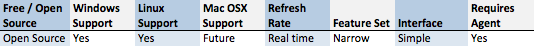
\includegraphics[width=110mm]{Competitors/OurSolutionSurvey}
\caption{General overview of our solution}
\end{figure}

%-----------------------------------------------------------------------------------------------------------------------------------------------

\section{Daemon performance testing}

Focusing on a lightweight daemon, our current implementation at standard refresh rates of 5 seconds for real-time and 50 seconds for each server message, will query all watchers every 5 seconds. 
With these settings, the Daemon, when compiled in Release mode with full optimizations on Windows, uses up 4.3-4.4MB of RAM at any moment in time, and a maximum of 0.1\% CPU when it queries the watchers, with a very common usage of 0\% - due to the fact that practically all of the daemon's threads sleep most of the time. The daemon's executable in this form is 602KB large, and only requires a simple settings text file along with it, which is under 1KB in size. 

There is no significant difference between this and an unoptimized, debugging version as far as resource usage go - the only one is seemingly 0.1MB more of RAM usage. However, the size of the executable on the disk is much larger for the unoptimized version, as this would take up 1985KB - three times the size of the optimized version.

How does the daemon behave with different refresh times - is it scaleable to watching all parameters using even faster refresh cycles, for users that might, in the future, want to see usage in true real-time?
Setting our real-time refresh rate to 1 second, from five, and our server (archiving) rate to five seconds, reveals that usage is practically the same - although 0.1\% CPU usage is more common, and it can spike to 0.2\%. 

Setting the real-time refresh to the extremely small value of 1 millisecond, much faster than any other real-time monitoring application can be used at (by comparison, the fastest setting on Windows' Task Manager is 500 milliseconds, and the default is 1 second), the CPU usage of the daemon is stable between 3.3\% and 4.5\%, with RAM usage being ofcourse still stable at 4.4MB. 

This indicates that, even at rates at which it is very probable that no one would need to use, especially for long periods of time, the daemon can still have a minimal impact on the system. This is clarified in Figure \ref{fig:DaemonEvalGraph}, which gathers a few more data points, and shows how even with exponential acceleration of the refresh rate, the CPU usage climbs very slowly:

\begin{figure}[H]
\centering
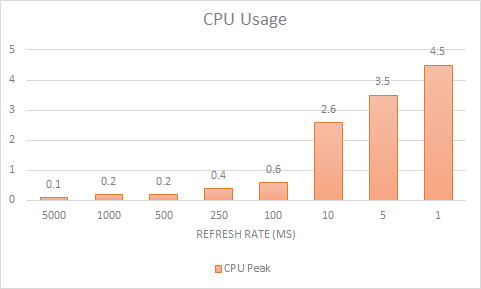
\includegraphics[width=110mm]{images/daemonusage}
\caption{Daemon CPU Usage\% over refresh rate}
\label{fig:DaemonEvalGraph}
\end{figure}

%-----------------------------------------------------------------------------------------------------------------------------------------------

\section{Server load testing}

We have reused the capabilities of our testing framework to create a working environment with thousands of users, hundreds of organisations and tens of thousands of daemons. To do so, we have written a testing application that is capable of dispatching multiple requests cuncurrently. The benchmark of success was how many people it correctly served and how well it managed to scale with an increasing load.

\begin{sidewaystable}
\begin{center}
  \caption{\textbf{Results} --- The last four rows represent how the problem scaled with respect to the previous in the group of three, how the time scaled, was the time scaling sublinear compared to the overall problem scaling, and whether the scaling was sublinear compared to the daemon scaling (always 10).}
  \label{tab:ServerEvalTab}
  \begin{tabular}{ | c | r | r | r || r || r | r | r | c | c | }
    \hline
      \rowcolor{DarkGrey}
     \textbf{Errors} & \textbf{No. Organisations} & \textbf{Users/org} & \textbf{Daemons/org} & \textbf{Time (ms)} & \textbf{Problem size} & \textbf{Problem scaling} & \textbf{Time scaling} & \textbf{sl scale overall} & \textbf{sl scale daemon} \\ \hline
      & 1 & 1 & 1 & 7 & 2 & - & - & - & - \\  
      \rowcolor{Grey}
      & 1 & 1 & 10 & 24 & 11 & 5.50 & 3.43 & 1 & 1 \\ 
      & 1 & 1 & 100 & 195 & 101 & 9.18 & 8.13 & 1 & 1 \\ 
      \rowcolor{Grey}
      & 1 & 10 & 1 & 26 & 11 & - & - & - & - \\  
      & 1 & 10 & 10 & 120 & 20 & 1.82 & 4.62 & 0 & 1 \\ 
      \rowcolor{Grey}
      & 1 & 10 & 100 & 852 & 110 & 5.50 & 7.10 & 0 & 1 \\  
      & 1 & 100 & 1 & 225 & 101 & - & - & - & - \\  
      \rowcolor{Grey}
      & 1 & 100 & 10 & 1020 & 110 & 1.09 & 4.53 & 0 & 1 \\ 
      & 1 & 100 & 100 & 8154 & 200 & 1.82 & 7.99 & 0 & 1 \\  
      \rowcolor{Grey}
      & 5 & 1 & 1 & 17 & 10 & - & - & - & - \\  
      & 5 & 1 & 10 & 123 & 55 & 5.50 & 7.24 & 0 & 1 \\  
      \rowcolor{Grey}
      & 5 & 1 & 100 & 996 & 505 & 9.18 & 8.10 & 1 & 1 \\  
      & 5 & 10 & 1 & 120 & 55 & - & - & - & - \\ 
      \rowcolor{Grey}
      & 5 & 10 & 10 & 568 & 100 & 1.82 & 4.73 & 0 & 1 \\  
      & 5 & 10 & 100 & 4402 & 550 & 5.50 & 7.75 & 0 & 1 \\  
      \rowcolor{Grey}
      & 5 & 100 & 1 & 1395 & 505 & - & - & - & - \\ 
      & 5 & 100 & 10 & 4991 & 550 & 1.09 & 3.58 & 0 & 1 \\  
      \rowcolor{Grey}
      & 5 & 100 & 100 & 40711 & 1000 & 1.82 & 8.16 & 0 & 1 \\  
      & 10 & 1 & 1 & 38 & 20 & - & - & - & - \\  
      \rowcolor{Grey}
      & 10 & 1 & 10 & 196 & 110 & 5.50 & 5.16 & 1 & 1 \\  
      & 10 & 1 & 100 & 2040 & 1010 & 9.18 & 10.41 & 0 & 0 \\  
      \rowcolor{Grey}
      & 10 & 10 & 1 & 249 & 110 & - & - & - & - \\  
      & 10 & 10 & 10 & 944 & 200 & 1.82 & 3.79 & 0 & 1 \\  
      \rowcolor{Grey}
     !!! & 10 & 10 & 100 & 161695 & 1100 & 5.50 & 171.29 & 0 & 0 \\
      & 10 & 100 & 1 & 2691 & 1010 & - & - & - & - \\  
      \rowcolor{Grey}
     !!! & 10 & 100 & 10 & 10699 & 1100 & 1.09 & 3.98 & 0 & 1 \\  
     !!! & 10 & 100 & 100 & 152464 & 2000 & 1.82 & 14.25 & 0 & 0 \\
    \hline
  \end{tabular}
\end{center}
\end{sidewaystable}

There is a lot of data in Table \ref{tab:ServerEvalTab}, so let us break it down. The first column tells whether all the tests have succeeded. The subsequent three columns are the test parameters. Then, there is the time it took to complete the tests. The rest of the table contains some basic analysis, like what is the total number of connections that is featured in the test case. Tests are grouped into small groups of three, where we increase the number of daemons tenfold. 

The testing scenario was the same for everything: we would prepopulate the database with the said number of organisations, users and daemons, then we would connect all the daemons to the server, executing basic commands, keep them alive and connect all the users. Having done that we would try to execute usual user behavior pattern: look at the whole list of daemons, for every single daemon then look up his historical monitoring information.

One of the initial findings from this test suite was that Linux has a limit to open file descriptors, which abstract sockets there. It turned out to be just above 1000, causing those tests to fail for some of the connections. This has dramaticaly increased the running time of them, since the server would try to accept the connection multiple times after certain timeouts. This has also meant, that with the current implementation and the server configuration it is impossible to reach the massive non-functional requirements that were described in Section \ref{nfrequirements}.

Overall, looking at the test results, we are rather satisfied with the way that the server scales. Despite having a concurrency bottleneck in the hub, the server sometimes manages to perform sublinearly in overall terms, and if you consider everything constant and that it is only daemons whose number is increasing tenfolds, then it is almost always sublinear. Bare in mind, that the server was run on only one core\footnote{\raggedright{}We have run the tests on an Arch Linux virtual machine, that had 512 MB of RAM and 1 2.3 GHz core available.}, so there was no benefit from the parallelism, only concurrency. Which is unfortunate, since the server could easily benefit from parallelism, knowing that there is no data sharing between goroutines until the point where we send the results.

In terms of performance, the server did consume 100\% of that CPU it run on. This was expected due to the way the tests were structured.

The tests were not ideal, though. Both the test suite and server ran on the same machine, which made it really easy to devise the test suite, but this setup significantly loses in realism to other options. There is no network delay and the machine is loaded by both server and tests, both holding hundreds of open connections. Ideally, the load test should be done on a server running in a believable environment, with a multicore CPU and parallelism turned on (it is off by default, since one has to be careful not to jeopardise the application performance with it, which is easier than it seems).

\subsection{Network load considerations}

At the current stage the system is not ready for heavy usage. The reason for that is that the amount of data scales linearly with the number of daemons that are being run. It can scale to a relatively large size, for example a list of 100 daemons weighs more than 4 KB. 

There is not much one can do to reduce this load, short of reducing the time resolution. One option might be introducing a compressed method for data transfer, similar to \texttt{XDR} that exists for \texttt{XML}, and which is used by Ganglia\footnote{\raggedright{}Ganglia's sourceforge page: \url{http://ganglia.sourceforge.net/}}, one of our many competitors in this field. The equivalent for \texttt{json} would probably be using \texttt{gzip} compression, however, that places a lot of computational strain on the components, and it is probably not too efficient for the shorter messages that constitute the absolute majority.

Another option would be to introduce our own compact data transfer protocol. However, it is doubtful that it will be significantly shorter than json, and it will definitely bring lots of various integration problems, as well as parsing bugs. In the end, this method would also probably require some sort of compression to be feasible.

In any case, it is very difficult to reason about the effectiveness of a protocol without having any data to back up the discussion. Hence, we would need to deploy the server into a realistic environment and carry out a technology spike regarding the transmission methods, refactor the code following the spike results. The current system does work for less strained usage scenarious, therefore it is a decent initial implementation.

\section{Summary}

We managed to iterate over our requirements based on client feedback and provide a solution that they were happy with. The functionality we implemented was mostly satisfactory, our daemon performance impressive, and while our server performance did not scale to as many users and organisations as we would like, our client reassured us that this would likely not be an issue in their work environment, likely using an instance of the server per small team. Overall, we are confident in calling our project a success, and our clients agree.

%===============================================================================================================================================

%===============================================================================================================================================

\chapter{Conclusion}

This chapter outlines some final thoughts on the project, describing how it went, what would we do if we had some more time and listing out our personal contributions.

%-----------------------------------------------------------------------------------------------------------------------------------------------

\section{Summary}

Our aim was to monitor server data remotely and in real time, with a simple and easy-to-use interface. After discussion with our client and technical evaluations we are satsfied that this is the case. While there is work we can do to improve our product, our current version is satisfactory and satisfying to have built.

A user can install and run a daemon on their machine and then use our web application to view graphs displaying CPU, RAM and network usage that update in real-time. The user can choose which of these metrics are being displayed at any given time, and can even query the server for past data over a user-specified date range. We even implemented the client requested feature where upon launching the application, graphs display some past information before updating in real-time, giving the user some instant context about how their servers have been performing.

%-----------------------------------------------------------------------------------------------------------------------------------------------

\section{Future Work}

\subsection{Future of the Client}

Like all the other components, the client needs a lot of future work. Firstly, as a primary task, its functionality can be expanded by introducing alerts and a daemon management system. The current chart implementation lacks navigation (history back and forward buttons). It would be useful if a user could navigate in the history charts because the library is not able to draw too many data points. Also, such navigation would be easier to use for the short ranges of dates than the datepicker.

Some communication related code should be refactored to support the new functionality. A proper testing approach should be applied to all the components of the client. Also, having a comparison view of the daemons could be useful for many users.

\subsection{Server refactoring}

The Server was developed from the echo-server, and some of its core functionality was poorly migrated. In particular, there is no sane reason for the connections to broadcast the message to the hub, from where it is then sent to the controller. It is in fact just a useless bottleneck; the connections should send the message directly to the controller, keeping things concurrent. We expect this to be a very significant boost in performance.

The handlers receive commands as Go structures, but they are ultimately responsible for checking, whether the command is valid. This includes many typechecks that in a sense pollute the code. Such checks should be avoidable by introducing a machine-readable documentation of the API, so that, in addition to parsing the \texttt{json}, \texttt{Go} could verify the command syntax. In addition to making the code more readable, this would allow current handler tests to be reduced to proper unit tests without losing too much in working guarantees.

There are virtually no security considerations in the current implementation, aside from minimum precautions against the server being broken completely by a bad command. In the real product, this, of course, should be changed. Passwords have to be hashed, and there has to be some precautions taken against spamming the server with messages. Currently, if a daemon chooses to send the server a message every 5 ms, it will gladly accept the message and store it in the database, wasting the space. And in general, there is no limit to how much pressure to the server a connection can apply, creating opportunity for even the simplest DDOS attacks to succeed. 

One additional interesting improvement that was planned, yet scrapped due to the lack of time, was introducing the different data resolutions for the historical monitoring information. It would manifest in the server storing older datapoints less frequently. For example, the present data might be stored in the 5 minute intervals, while yesterday's information might be reduced to one datapoint every hour and so on. This would make the application actually feasible in the long run. It requires periodical data transfer to lower resolution collections, or, preferably, merging the old documents in the same collection, since this would require no other code change. This is also one of the ways to implement the high level overview of the historical data that our client at J.P. Morgan deemed interesting, since reducing the resolution will ultimately give a very abstract report.

\subsection{Implementation of missing Server functionality}

The server lacks the support of generating alerts, that can be easily introduced. It also does not provide the functionality that we deemed too obvious to focus on, like registering your company or a user within one. While not particularly interesting, these features are essential to any real product and hence have to be implemented in one.

\subsection{Further Daemon development}

The daemon, while exhibiting a good overall design with very useful features already implemented, can become much better through a few improvements.

One simple improvement would be to provide options regarding how data is collected. Currently, a data point is retrieved from the watchers with each refresh cycle, and the data from that point is sent directly to the connected clients. When the server refresh cycle reaches its point of action, the latest datapoint is also sent to the server. This is a good approach that also keeps resource usage to a minimum, but another option would be very useful for many users: averaged datapoints. This would make the watchers collect data more often, perhaps at a refresh rate set by the user, and the manager would average all collected datapoints before sending it as one point to the clients or server. The collected datapoints would then be cleared for the next cycle. This would allow for more robust monitoring, coming with the cost of more resources.

Another very useful feature would be simplifying the addition of more watchers even more, by modifying the daemon to load the watchers from external dynamic libraries. This way, watchers could be developed completely separate from the daemon, not requiring access or modifications to the daemon's code.

Other additions and improvements that could be done are some general restructuring of the watcher classes to avoid some unnecessary code, and refactoring for certain parts of the main manager, which would benefit from being moved into dedicated parts of the daemon to be used from the main manager.

%-----------------------------------------------------------------------------------------------------------------------------------------------

\section{Reflection}

Every single member of the team came away from this project learning something new. It was a fantastic opportunity to learn new and cuting edge languages and technologies, as well as putting into practice project management methods that will be essential outside of university. It was extremely satisfying to build a complete application from the ground up and have it be a success, knowing that we each made it happen.

If we were to change anything about how we tackled the project, it would probably be enforcing attendance more strictly at meetings and providing progress reports. The separation of our components had its benefits discussed at length in this dissertation, however, it often resulted in team members working on their own and not thinking to discuss progress as often as we perhaps should have.

%-----------------------------------------------------------------------------------------------------------------------------------------------

\section{Contributions}

\textbf{Sean Jakobsen} coordinated the dissertation writing, conducted market research, drew the design prototypes and worked on the client application. 

\textbf{Maksim Solovjov} conducted market research, liasoned with our clients at J.P Morgan and wrote the Go server and database components.

\textbf{Aleksandrs Sidlovskis} drew up our architectural diagram, drafted the API and worked heavily on the client application.

\textbf{Gabriel Alexandru Susanu} developed the platform-specific daemons and their ability to monitor the different metrics needed.

\textbf{Supanat Auengsirirat} wrote our help manual and assisted with some daemon functionality.

%===============================================================================================================================================

%===============================================================================================================================================

\begin{appendices}

\chapter{Preliminaries}
\label{prelim}

Here are the necessary terms that a reader may not be familiar with. More knowledgeable readers may feel free to skip this section of the report.

\textbf{Performance monitoring} -- observing the statistics of some system, which relate to how well the system runs. For example monitoring the CPU load in order to ensure that it does not exceed some healthy threshold.

\textbf{Cloud-based solution} -- the program that is provided as a service on some external machines (which might be owned by a separate organisation) accessible via internet.

\textbf{Client (Application)} -- in our case, a user-facing application, running in a user’s browser.

\textbf{Server} -- a computation-intensive application that serves the client application to the user and provides the gateway to the database.

\textbf{Daemon} -- a monitoring application, running on the machine that is to be monitored, storing the performance metrics and sending them to the Server and Client.

\textbf{Relational database} -- a database, modelled by creating entities and expressing their relationships to each other. Interaction with the stored data is governed by relational algebra.

\textbf{NoSQL database} -- an alternative to the relational database, which allows easy horizontal scaling (can accommodate more data), in our case (MongoDB) expressed via collections of documents with no enforced schema (blueprint).

\textbf{WebSocket} -- a protocol, that allows simultaneous bidirectional communication over a single TCP connection. To put it in simple terms, it lets a user to both send and receive data in real-time without the overhead of making multiple ``internet'' connections.

\textbf{Concurrency} -- splitting work into independent chunks, that can be done in any particular order, allowing switching from one task to another should the first one temporarily stall.

\textbf{Parallelism} -- executing multiple concurrent tasks at the same time. 

\textbf{Goroutine} -- a concept in Go, lightweight thread of sorts. The ``physical'' threads in the OS execute program instructions concurrently. A goroutine represents such a thread, but it is actually mapped to one by the Go runtime that manages a thread pool. Hence, Go is an example of managed concurrency.

\textbf{Runtime} implements core language functionality, and sometimes serves higher level functions.

\textbf{Refactor} -- rewrite, in order to improve the quality of the code without changing its output.

%===============================================================================================================================================

%===============================================================================================================================================

\chapter{Team organisation}

At the beginning we thought that we will have a laisses faire approach to the development within our team, however, soon some specific roles formed within it, influenced by the very modular design of the whole system. We had one person driving the design and helping with the client side, one person working on a client side solely, one person working on the server side, one person working on daemons, and finally one person on the user manual duty. These roles then stayed for the duration of the whole project.

We would usually have three formal weekly meetings in our team: on Tuesdays to drive the development, on Thursdays with the supervisor to catch up on what was done and ensure that we are on track, and straight after that yet another short team meeting to address the supervisors feedback. Meetings were the place where most of the decisions would have been made, thus they were extremely important to the whole development process.

In addition to that, we have used plenty of other communication mediums. We had a facebook group where we would post current headlines. During the heat of the development process we would use skype conference calls if we were working remotely. In order to keep track of current issues we had a Kanban board online. Finally, we had exchanged our phone numbers with each other so that we could be contacted directly in case of emergency.

%===============================================================================================================================================

%===============================================================================================================================================


\chapter{Full API documentation}
\label{API}

This documentation, of course, does not live up to the professional standards. However it is for the most part a valid \texttt{json}, allowing to infer the types of the messages, as well as reuse them in tests straight away. 

\lstinputlisting{src/api.txt}

%===============================================================================================================================================

%===============================================================================================================================================


\chapter{User Manual}

This version of the application currently supports monitoring of Linux and Windows platforms.

It allows you to monitor three metrics: CPU, RAM and network usage. The table below show the units of each of these. 

\begin{center}
  \begin{tabular}{ | c | c | }
    \hline
     \textbf{Metric} & \textbf{Unit} \\ \hline
        CPU & percentage \\ \hline 
        RAM & byte \\ \hline 
        NET(Network) & byte/sec \\ \hline 
  \end{tabular}
\end{center}

The application is accessed through the browser, keeping things as simple and accessible as possible. There are two main views; the main dashboard view shows graphs updating in real time for your systems, and the second one allows you to query historical data. When you log in to the application, you will be shown the main dashboard.

\section{Home view --- the main dashboard}

\begin{figure}[H]
\centering
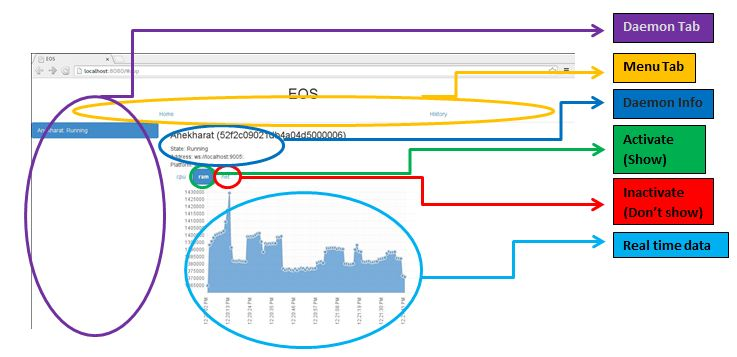
\includegraphics[width=110mm]{Manual_Images/realtime_data.JPG}
\caption{Real-time Data Page}
\label{fig:Real-time Data Page}
\end{figure}

Figure \ref{fig:Real-time Data Page} shows that both the home view and history view will have a \textbf{daemon list} and \textbf{menu tab}. The daemon list will show all the daemons running on your systems where you can select the required daemon and get information specific to its system on the right. The menu tab simply allows you to switch between the main view and the history view.

The home view will show graphs updating in real time depending on what data you have currently selected to monitor. Currently, this version of the application is able to monitor CPU, RAM and network usage. As seen in figure \ref{fig:Real-time Data Page} \textbf{real time data} the x-axis of graphs represents time and the y-axis is the value dependant on the selected metric. You can select the type of metric to display by clicking the appropriately named button at the top of the view. The button colour will toggle between blue and white, where if a button is blue you are receiving data about that metric and if it is white you are not.

\section{History view}

\begin{figure}[H]
\centering
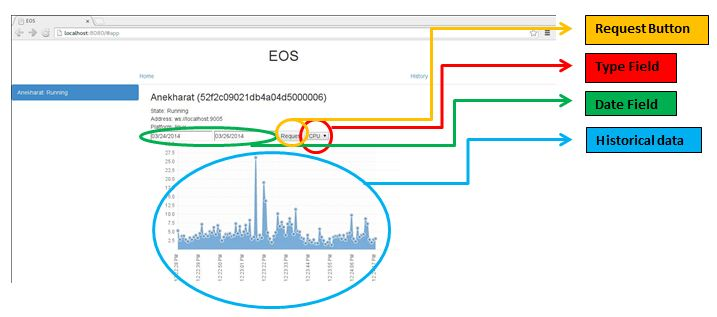
\includegraphics[width=110mm]{Manual_Images/historical_data.JPG}
\caption{Historical Data Page}
\label{fig:Historical Data Page}
\end{figure}

In the history view, you can receive a graphical view of your past data for any of your monitored systems, simply by choosing a date range and a metric. The \textbf{date field} is where you can select the start and end date and the metrics can be chosen from a combo box in the \textbf{type field}. When you're ready, click on the \textbf{request button} and the \textbf{historical data} will be shown as a graph. 

%===============================================================================================================================================

%===============================================================================================================================================

\end{appendices}

\bibliographystyle{IEEEtran}
\bibliography{TeamM_Bibliography}

\end{document}